%\documentclass[12pt,draftcls]{ucdavisthesis}
\documentclass[12pt]{ucdavisthesis}

% PLEASE READ THE MANUAL - ucdavisthesis.pdf (in the package installation directory)

%%%%%%%%%%%%%%%%%%%%%%%%%%%%%%%%%%%%%%%%%%%%%%%%%%%%%%%%%%%%%%%%%%%%%%%%
%                                                                      %
%               LATEX COMMANDS FOR DOCUMENT SETUP                      %
%                                                                      %
%%%%%%%%%%%%%%%%%%%%%%%%%%%%%%%%%%%%%%%%%%%%%%%%%%%%%%%%%%%%%%%%%%%%%%%%

%\usepackage{bookmark}
\usepackage[us,nodayofweek,12hr]{datetime}
\usepackage{graphicx}
\usepackage{wrapfig}
\usepackage[labelfont=bf,font=scriptsize]{caption}
%\usepackage[square,comma,numbers,sort&compress]{natbib}
%\usepackage{hypernat}
% Other useful packages to try
%\usepackage{amsmath}
%\usepackage{amssymb}
%
% Different fonts to try (uncomment only fontenc and one font at a time)
% (you may need to install these first)
\usepackage[T1]{fontenc} %enable fontenc package if using one of the fonts below
\usepackage[adobe-utopia]{mathdesign}
%\usepackage{tgschola}
%\usepackage{tgbonum}
%\usepackage{tgpagella}
%\usepackage{tgtermes}
%\usepackage{fourier}
%\usepackage{fouriernc}
%\usepackage{kmath,kerkis}
%\usepackage{kpfonts}
%\usepackage[urw-garamond]{mathdesign}
%\usepackage[bitstream-charter]{mathdesign}
%\usepackage[sc]{mathpazo}
%\usepackage{mathptmx}
%\usepackage[varg]{txfonts}
\usepackage[final]{pdfpages}
\usepackage{color, colortbl}

\hyphenation{dis-ser-ta-tion blue-print man-u-script pre-par-ing Phy-lo-gen-etic Pro-kar-y-ot-ic as-so-ci-at-ed} %add hyphenation rules for words TeX doesn't know


%\renewcommand{\rightmark}{\scriptsize A University of California Davis\ldots \hfill Rev.~\#1.0 \quad Compiled: \currenttime, \today}
% a fancier running header that can be used with draftcls options

%%%%%%%%%%%%%%%%%%%%%%%%%%%%%%%%%%%%%%%%%%%%%%%%%%%%%%%%%%%%%%%%%%%%%%%%
%                                                                      %
%        DOCUMENT SETUP AND INFORMATION FOR PRELIMINARY PAGES          %
%                                                                      %
%%%%%%%%%%%%%%%%%%%%%%%%%%%%%%%%%%%%%%%%%%%%%%%%%%%%%%%%%%%%%%%%%%%%%%%%

\title          {Structure, Variation, and Dynamics of the Root-Associated Microbiota of the Crop Plant Rice}
%Exact title of your thesis. Indicate italics where necessary by underlining or using italics. Please capitalize the first letter of each word that would normally be capitalized in a title.

\author         {Joseph Andrew Arthur Edwards}
%Your full name as it appears on University records. Do not use initials.

\authordegrees  {B.S. (Virginia Polytechnic Institute and State University) 2011}
%Indicate your previous degrees conferred.

\officialmajor  {Plant Biolgy}
%This is your official major as it appears on your University records.

\graduateprogram{Plant Biology}
%This is your official graduate program name. Used for UMI abstract.

\degreeyear     {2016}
% Indicate the year in which your degree will be officially conferred.

\degreemonth    {December}
% Indicate the month in which your degree will be officially conferred. Used for UMI abstract.

\committee{Venkatesan Sundaresan, Chair}{Siobhan Brady}{Kate Scow}{}{}
% These are your committee members. The command accepts up to five committee members so be sure to have five sets of braces, even if there are empties.

%%%%%%%%%%%%%%%%%%%%%%%%%%%%%%%%%%%%%%%%%%%%%%%%%%%%%%%%%%%%%%%%%%%%%%%%

%\copyrightyear{2020}
%\nocopyright

%%%%%%%%%%%%%%%%%%%%%%%%%%%%%%%%%%%%%%%%%%%%%%%%%%%%%%%%%%%%%%%%%%%%%%%%

\dedication{\textsl{To my family \\
            For your inexhaustible love and support}}

%%%%%%%%%%%%%%%%%%%%%%%%%%%%%%%%%%%%%%%%%%%%%%%%%%%%%%%%%%%%%%%%%%%%%%%%

\abstract{Soil microbes are important mediators of plant nutrition, growth, and resistance to biotic and abiotic stresses, thus understanding the composition and dynamics of plant root-associated microbial communities is of importance to scientists and farmers. Plants acquire root-associated microbiota that are distinct from that of the surrounding soil. In this thesis I detail general characteristics of the rice root-associated microbiota. 

In the first chapter I introduce the importance of both animal and plant microbiota and I discuss the technological breakthroughs that have allowed scientists to study complex microbial ecosystems. 

In the second chapter, I present the results of a study characterizing the rice root-associated microbiota across three root compartments: the soil adjacent to the root (the rhizosphere), the root surface (the rhizoplane), and the root interior (the endosphere). I present how the composition of the microbiota in these compartments varies across soil type, cultivation practice, and host plant genotype. 

In the third chapter, I present the results of a study characterizing the rice root-associated microbiota compared to diverse species of both crop plants and native plants growing in the same environment as rice. The results suggest that rice assimilates a unique root-associated microbiota and that plant phylogenetic variation cannot fully explain microbiota variation between the tested host plants. A comparison of the root-associated microbiomes of rice with microbiota of soil from cultivated fields and non-cultivated soils, suggests that rice cultivation changes the overall soil microbiome in rice fields not only through agricultural inputs and water submergence, but also through specific enrichment of microbial taxa by rice plants. 

In the fourth chapter, I demonstrate how the rice root-associated microbiota shifts across the lifecycle of the host plants under field conditions. We find that the composition of the microbiome shifts throughout vegetative growth until the initiation of reproductive growth, whereupon the microbiome stabilizes. These results suggest that plants select for different microbiota as they undergo developmental changes from germination to reproduction. 

I present concluding remarks on the various models of microbiota acquisition and discuss future implications of this research in the fifth and final chapter of this dissertation.
}

%%%%%%%%%%%%%%%%%%%%%%%%%%%%%%%%%%%%%%%%%%%%%%%%%%%%%%%%%%%%%%%%%%%%%%%%

\acknowledgments{Acknowledgements to those who helped you get to this point. They should be listed by chapter when appropriate.}

%%%%%%%%%%%%%%%%%%%%%%%%%%%%%%%%%%%%%%%%%%%%%%%%%%%%%%%%%%%%%%%%%%%%%%%%

% Each chapter can be in its own file for easier editing and brought in with the \include command.
% Then use the \includeonly command to speed compilation when working on a particular chapter.
%%% \includeonly{ucdavisthesis_example_Chap1}

\begin{document}

\newcommand{\bibfont}{\singlespacing}
% need this command to keep single spacing in the bibliography when using natbib

\bibliographystyle{plain}
%many other bibliography styles are available (IEEEtran, mla, etc.). Use one appropriate for your field.

\makeintropages %Processes/produces the preliminary pages

\chapter{Introduction}
\section{The beginnings of microbiology and microbial ecology}
%
For centuries, humans have been curious to understand the unseen organisms that surround them: this is the basic objective of microbial ecology. Up until the 17th century, however, prominent scientists were naive to the lifeforms that could not be observed with the naked eye. The field of microscopy began to expand when the Englishman Robert Hooke developed one of the first compound microscopes and published the book \textit{Micrographia} \cite{Hooke1665} in 1665 with detailed drawings of never before observed images of magnified organisms and structures. It was in this book that he coined the term cell after observing plant cells from cork tissue. He based this term on the resemblance to the walled structure in honeycomb. Unfortunately, very little is known of Hooke's career and accomplishments (there does not even exist a portrait of him) due to his falling out with contemporary scientists of prominence, namely Sir Isaac Newton \cite{Espinasse1962}.	

Hooke's microscopy work inspired others, however. Antonie van Leeuwenhoek took an interest in Hooke's Micrographia in order to apply microscopy to his business of owning and operating a drapery \cite{Dobell1932}. Leeuwenhoek, a Dutch businessman, was intent to use the finest quality thread and fabric for his work, and believed he could have an advantage over his competitors if he were to use an instrument with higher magnification than modern magnifying glasses to inspect the material for imperfections. Leeuwenhoek was skilled at grinding lenses from glass and was able to craft microscopes with 200X magnification, thus surpassing the capability of the best microscopes at the time, the most powerful of which had 30X magnification. He began to discover many microscopic structures which had yet to be observed. Most notable among these observations were blood cells, sperm cells, and protists and algae from pond water. After he would record his observations, he would write letters in Dutch to the Royal Society of London, which would be translated to English or Latin and then published by the society. In 1683, Leeuwenhoek wrote a letter to the Royal Society detailing the life forms which he had observed within plaque sampled from between his teeth. He wrote of the motility and the dense occurrence of at least two types of ``animalcules'', what we now know as bacteria. These observations led to the emergence of the microbiology and microbial ecology fields.

\section{The foundation of modern microbial ecology experiments}
%
Microbial ecology is the broad study of microbial organisms in their natural environments \cite{Atlas1986}. One of the primary objectives of microbial ecology is to understand the complete diversity of microbial organisms cohabitating a single environment. This objective includes understanding the taxonomic classification of the detectable microbes. Culturing individual microbial isolates from environmental samples, which was established by Robert Koch in the late 19th century \cite{nobel1967}, was a promising technique for surveying the microorganisms present in each sample. However, it was found apparent that the diversity levels capable of being cultured on media were underwhelming compared to the diversity of microorganisms observed under a microscope. Specifically, in soil, <1\% of microorganisms are capable of being cultured under laboratory conditions \cite{Hugenholtz1998}. Thus culturing isolated microbes is currently a fruitless task for surveying overall diversity, while microscopy will give little to no answers about the taxonomic information of the observed microbes. 

In order to get a better grasp of the microorganisms present in environments and to what taxonomic classifications they belong, scientists turned to culture-independent surveys \cite{Hugenholtz1998}. One groundbreaking and seminal technique was the use of 16S ribosomal RNA to classify microorganisms phylogenetically by Carl Woese and colleagues. Woese, in the mid 1970's, was skeptical of the dogma that all organisms separate into 2 domains solely based on the presence or absence of a nucleus, i.e. eukaryotes and prokaryotes. In his seminal study \cite{Woese1977}, Woese complained that ``Dividing the living world into Prokaryotae and Eukaryotae has served, if anything, to obscure the problem of what extant groupings represent the various primeval branches from the common line of descent.'' He made this complaint because using presence or absence of nuclei as a classifier of domain is not a phylogenetic measure, and thus scientists cannot resolve evolutionary relationships in any meaningful way using this metric. Woese and his colleague, John Fox, proved their point by comparing 16S rRNA sequences found in prokaryotic microorganisms to 18S rRNA sequences from eukaryotes (the homologous eurkaryotic rRNA to 16S rRNA in prokaryotes) \cite{Woese1977}. They used 16S rRNA as the phylogenetic marker because they needed a biological molecule that was conserved across the tree of life, slowly evolved over time, and was easily extractable from cells. No known protein fit these descriptions at the time. They found that, through analysis of 16S rRNA, prokaryotic organisms had 2 distinct lineages which were similarly distant from each other as each lineage was to eukaryotes. They termed these lineages as eubacteria and archaebacteria. Not only did Woese and Fox discover a new domain of life, but they laid the groundwork for using the phylogenetically conserved 16S rRNA subunit as a marker for topologically describing the tree of life.

Woese conducted his fundamental studies on cultured organisms. Norman Pace, a colleague of Woese, began to apply 16S rRNA sequencing to unculturable organisms to identify evolutionary lineages of uncharacterized bacteria and archaea \cite{Pace1986}. The scientific community soon adopted his approach and the vast topology of the tree of life began to fill in. In the 1980's, when these studies were taking place, DNA sequencing was a tedious, non-trivial process. Two decades later, DNA sequencing technology reached major breakthroughs causing the rapid expansion of genomic studies and importantly microbial ecology studies.

\section{The rise in modern microbial ecology}
%
Relatively recently, the use of culture-independent techniques to study microbial community structure has been rebranded under new field names. The Google search terms ``microbiome'' and ``microbiota'' are trending over the last decade and are still rising. The search term for ``microbial ecology'', on the other hand, is decreasing. I will define the terms microbiome and microbiota and give a few potential reasons as to why these fields have expanded in popularity.

\begin{figure}[tbh]
\centering
\includegraphics[width=2.75in]{Figures/intro_fig1}
% where an .eps filename suffix will be assumed under latex,
% and a .pdf suffix will be assumed for pdflatex
\caption[Figure 1.1]{Popularity of Google searches for terms related to microbial ecology over the last decade. Data was collected from Google Trends (https://www.google.com/trends/).}
\label{Figure 1.1}
\end{figure}

A microbiota is the complete catalog of microorganisms inhabiting an environment. The definition of the environment can range depending on the study system, but typically the term microbiota refers to microbial communities that are associated with a multicellular host. The study of the human gut microbiota by Jeffrey Gordon's lab has led to growing interests in host-associated microbiomes. Peter Turnbaugh, Ruth Ley and Fredrik Backhed, all members of Gordon's Laboratory, drew a direct connection between the gut microbiota and the host species' physiology and phenotype \cite{Turnbaugh,Backhed,Ley2005}. They showed that lean and obese mice hosted significantly different communities of microbes in their guts and when an obese mouse gut microbiota was inoculated into lean mice or germ free mice (i.e. mice that have no microbes in their gut) that the recipients rapidly gained body fat. These studies definitively showed that the gene content of the microbiota residing in a host animal's gut, i.e. the microbiome, has the ability to significantly influence the host's physiology and health. These studies were instrumental for initiating the Human Microbiome Project \cite{Turnbaugh2007} as well as providing a significant motivation for studying all other host-associated microbiomes, including plant microbiomes.

\begin{figure}[tbh]
\centering
\includegraphics[width=2.75in]{Figures/intro_fig2}
% where an .eps filename suffix will be assumed under latex,
% and a .pdf suffix will be assumed for pdflatex
\caption[Figure 1.2]{Standard workflow for profiling microbial communities from environmental DNA.}
\label{Figure 1.2}
\end{figure}

While biological advances drew a considerable amount of interest to the field of microbiomes, sequencing capability still posed technical barriers for understanding host-associated microbial communities in depth. 16S rRNA sequencing was the method of choice for profiling microbial communities but researchers were burdened by the process of cloning 16S rRNA PCR amplicons into plasmids, cloning into Escherichia coli, and using Sanger sequencing to survey microbial diversity within samples. This method is relatively tedious, very low throughput, and expensive. At the time, a standard study would profile 300-400 different clones for each sample. Next generation sequencing again revolutionized the technical aspect of microbial ecology field. The first application of pyrosequencing to 16S rRNA sequencing was by Sogin et al in 2006 \cite{Sogin2006}. They were able to sequence over 119,000 16S rRNA sequence tags and importantly they were able to barcode separate samples into a single sequencing run. Pyrosequencing became the preferred method for researchers investigating microbiomes, but this technology would soon be surpassed. Illumina sequencing, which had previously not been applicable to profiling 16S rRNA fragments due to read length limitations, began to emerge as the standard method for sequencing once the MiSeq platform was introduced in 2011 \cite{Caporaso2011}. Compared to the previous iteration of Illumina chemistry, the MiSeq platform allowed for greater read lengths, while maintaining the high throughput standard with Illumina. The general workflow for community profiling using 16S rRNA gene sequencing is displayed in Figure 2.

\section{Plant Associated Microbiomes}
%
The impact of host-associated microbial communities on animal health is a robust area of research. Investigators are similarly interested in plant-associated microbiota. As sessile organisms, plants rely on their environment for the uptake of critical nutrients \cite{Epstein1971}. Co-habitating the soil with plants are thousands of different bacterial and archaeal strains, some of which are known to aid host plants in tolerating otherwise inhospitable conditions. For example, the genus Lupinus in the Fabaceae family, thrives in nitrogen poor soil where other plants struggle to survive. The lupine received its name because it was thought to act as a wolf, plundering nutrients in the soil and thus making the environment unfavorable for the growth of other plants \cite{Austin2004}. This hypothesis was false. In fact, lupines and other members of the Fabaceae family, form symbiotic relationships with nitrogen fixing soil bacteria thereby allowing them to survive otherwise nitrogen limited conditions \cite{Vance2001}. This is an important and widespread example of how plants form beneficial relationships with soil microbes.
	
Plants also rely on soil microbes to survive attacks from pathogens \cite{Berendsen2012,Bulgarelli2012}. In some cropping systems, such as sugar beet and wheat, continuous monoculture cultivation of soil leads to reduced loss of yield from pathogen infection \cite{Hornby1983}. It was found that this phenomenon is transmissible to other, non-suppressive soils and that the effect is lost upon pasteurization at $80\,^{\circ}\mathrm{C}$, thus suggesting that the mechanism is biological in nature \cite{Hornby1983}. Mendes et al. tested the root-associated bacterial communities between sugar beet seedlings grown in soils suppressive to \textit{Rhizoctonia solani} infection and soils conducive for infection (sampled from the margin of the fields where suppressive soils were located) \cite{Mendes2011}. They found that no single bacterial or archaeal strain was responsible for the difference in microbial community structure between suppressive and conducive soils. Many of the microbial strains they detected differed in relative abundance between the soils, mainly within the Gamma and Beta Proteobacterial classes. These results were instrumental in demonstrating how broader microbial communities, i.e. the root microbiota, are important for soil and plant health.

Because soil microbial communities were found to impact plant health, deep characterizations of the plant root microbiota began to take place. In 2012, two groups published studies characterizing the root-associated microbiota of \textit{Arabidopsis thaliana} \cite{Bulgarelli2012,Lundberg2012,}. These studies found that the consortia of microbes inside of the root (the endosphere) is significantly different and of lower diversity than the microbial communities in the soil adhering to the root (the rhizosphere). Each study found that variability in microbial community structure between different soils is also reflected in the root-associated microbial assemblages of the plants grown in the respective soils. The studies found plant genotype to have a small but significant effect on the microbial communities associated with the roots. It was later found in rice that there is a third discernible niche on the rhizoplane (the root surface) and that these microbial communities are intermediate in composition between the rhizosphere and endosphere \cite{Edwards2015}. A longitudinal study of early microbiome acquisition in rice detailed the dynamic changes in microbiota composition within the rhizosphere, rhizoplane, and endosphere compartments \cite{Edwards2015}. Together this data suggested a three-step model for microbiota assembly in the root: microbes are first attracted to the roots in the rhizosphere, perhaps by root exudates, after which a select set of microbes can attach to the rhizoplane and a subset of rhizoplane attached microbes can enter the root endosphere.

Open questions still remain for the plant root-associated microbiota. Functionally, there are only limited examples of how root associated bacterial and archaeal communities may impact plant fitness. Further studies are needed to assess how the root-associated microbiota may aid plants in tolerating abiotic and biotic stresses. Once a better understanding of how microbiomes may help to protect plants from various stresses is attained, researchers are intent to leverage crop genetics to breed for beneficial root microbiotas. Because intraspecies genetic variation has a minimal impact on the root-associated microbiota, it is of importance to better understand how host interspecies variation impacts the root-associated microbiome and what physiological traits are causal of microbiome divergence between plant species. It is also critical to understand how root associated microbial communities change over the life cycle of the host plant. Plants face different nutritional requirements at various stages of their lives, but it is yet to be characterized how root-associated microbial communities shift over the growing season and how these potential changes are tied to plant developmental shifts. 

This thesis is separated into three research chapters. In the first chapter, I characterize the root-associated microbiota of rice plants and quantify the factors affecting root assemblages. In the second chapter, I characterize how the rice root microbiota differs from other crop species as well as how the rice root microbiota differs from native plants growing in the same flooded environment. In this chapter I also show how continuous and intensive cultivation of rice enriches for a soil microbiota with rice specific microbes. In the final chapter, I demonstrate the dynamics of the root-associated microbiota over the life cycle of the rice plant and how the abundances of specific microbial taxa are tuned by the developmental stage of the host plant.
\chapter{Structure, variation, and assembly of the root-associated microbiomes of rice}

Joseph Edwards\footnote[1]{Department of Plant Biology, University of California, Davis}, Cameron Johnson$^1$, Christian Santos$^1$, Eugene Lurie$^1$, Natraj Podishetty$^1$, Srijak Bhatnagar\footnote[2]{Department Medical Microbiology and Immunology, University of California, Davis}, Jonathan A. Eisen$^2$ and Venkatesan Sundaresan$^1$

\section{Abstract}
Plants depend upon beneficial interactions between roots and microbes for nutrient availability, growth promotion, and disease suppression. High-throughput sequencing approaches have provided recent insights into root microbiomes, but our current understanding is still limited relative to animal microbiomes. Here we present a detailed characterization of the root-associated microbiomes of the crop plant rice by deep sequencing, using plants grown under controlled conditions as well as field cultivation at multiple sites. The spatial resolution of the study distinguished three root-associated compartments, the endosphere (root interior), rhizoplane (root surface), and rhizosphere (soil close to the root surface), each of which was found to harbor a distinct microbiome. Under controlled greenhouse conditions, microbiome composition varied with soil source and genotype. In field conditions, geographical location and cultivation practice, namely organic vs. conventional, were factors contributing to microbiome variation. Rice cultivation is a major source of global methane emissions, and methanogenic archaea could be detected in all spatial compartments of field-grown rice. The depth and scale of this study were used to build coabundance networks that revealed potential microbial consortia, some of which were involved in methane cycling. Dynamic changes observed during microbiome acquisition, as well as steady-state compositions of spatial compartments, support a multistep model for root microbiome assembly from soil wherein the rhizoplane plays a selective gating role. Similarities in the distribution of phyla in the root microbiomes of rice and other plants suggest that conclusions derived from this study might be generally applicable to land plants.\footnote[3]{All supplementary material and datasets can be found with the online version of this article: \url{http://www.pnas.org/content/112/8/E911}.}
\includepdf[pages=-]{PNASEdwards.pdf}
\chapter{The impact of host interspecies diversity on the root associated microbiome and potential implications in agriculture.}

Joseph Edwards\footnote[1]{Department of Plant Biology, University of California, Davis}, John Kilmer\footnote[2]{College of Agriculture and Technology, Arkansas State University}, Christian Santos$^1$, Bao Nguyen$^1$, Gregory Phillips$^2$, and Venkatesan Sundaresan$^1$

\section{Abstract}

Plant roots assemble a distinct root-associated microbiota from the soil which can contribute beneficial properties to plant growth and performance. Previous studies have indicated that root-associated microbiomes are mainly constrained by environmental factors that act upon the broader soil microbial communities and that various root compartments pose as different niches for microbial colonization with the rhizosphere hosting the highest diversity of microbes and the root endosphere hosting the least. It was consistently found across various plant microbiome studies that genetic diversity within a host plant species contributes a minimal proportion of variance to root-associated microbiome differences. Thus, we were interested in quantifying the effect of host species specificity on root-associated microbiomes and whether this effect outweighs microbiome diversity within host species. We compiled published datasets from various plant microbiome studies and found that the environment that various host species are growing in is the largest determinant of root-associated microbiome structure and that rice has a relatively unique microbiome, presumably because it is cultivated under flooded (i.e. anaerobic conditions). To better understand how root-associated microbiomes vary across host plant species within a single environment, we sampled the roots of native plant species from a rice field along with roots from rice plants. We found host specificity to be a large factor contributing to microbiome variation and that rice plants host a larger proportion of methanogenic archaea than native plants growing in the same environment. The rhizosphere microbiome of rice was significantly more similar to unplanted soil microbial communities than were the rhizosphere microbiomes of native plants. By comparing rice plants grown in rice field soil vs rice plants grown in soil which has never cultivated rice, we established that this observation was at least in part due to continuous rice cultivation establishing a microbiome more similar to the rice rhizosphere. Together, these results indicate that different host plants acquire largely dissimilar root-associated microbiomes and that when rice is grown in dense monoculture, it shifts the overall soil microbiome to be more resemblant of the rice rhizosphere microbiome.

\section{Introduction}
Land plants growing in soil interact with a vast array of microbial diversity via their roots. Individual soil microbes have been shown to provide plants with beneficial effects including general growth promotion, pathogen exclusion, and protection against abiotic stresses \cite{Berendsen2012}. Plant-associated microbes, however, do not act in isolation and are part of a broader interconnected community, collectively known as the rhizosphere or root-associated microbiome \cite{Bulgarelli2013}. Harnessing the beneficial properties of the root-associated microbiome is of agricultural and biotechnological interest, yet the parameters governing their assembly are not fully understood \cite{Bulgarelli2013}. 

Plant roots host microbiomes that are distinct from the surrounding soil. Furthermore, root-associated microbiomes differ in composition between the rhizosphere and the root endosphere, with the latter having a significantly reduced microbial diversity than the former \cite{Lundberg2012,Bulgarelli2012,Edwards2015,Peiffer2013,Wagner2016,Zarraonaindia2015}. Genotypic diversity within a host plant species has a significant role in shaping the root-associated microbiome \cite{Lundberg2012,Wagner2016,Peiffer2013,Edwards2015}. It was recently reported that root-endosphere enriched microbiomes of Arabidopsis relatives are compositionally distinct in only a few taxonomic members, and the patterns of these differences are contradictory to host species phylogeny \cite{Schlaeppi2014}. Consistent with other studies, the microbiome variance partitioned to plant genotype was largely overshadowed by the variance partitioned to environmental factors (i.e. soil type, batch, field location and treatments), suggesting that plants from different, but related, species assemble a largely taxonomically conserved microbiome derived from a subset of the soil microbiome reservoir, which is affected by various environmental factors.

Asian rice (\textit{Oryza sativa}) is primarily cultivated under flooded conditions, a growth habit unique for cereal crop plants. We have previously characterized the rice root-associated microbiome, finding that root-associated microbiomes can be separated into 3 spatially and compositionally distinct compartments: the rhizosphere, the rhizoplane, and the endosphere. Rice genotype, despite including another cultivated rice species in this study (\textit{Oryza glaberrima}), was a very small explanatory variable for root-associated microbiome differences. These results suggest that interspecies variation between domesticated members of the \textit{Oryza} genus minimally affects the root-associated microbiome; however, it is unknown how root-associated microbiomes vary outside of the \textit{Oryza} genus when grown under the same flooded conditions. In this study, we sought to characterize the rice root-associated microbiome compared to other plant species.

\section{Results}
\subsection{Root-associated microbiomes are influenced by environmental conditions.}
To examine interspecies variation among root-associated microbiomes, we compiled microbiome sequencing data from 5 published datasets (Table 3.1). Primer choice during 16S rRNA gene sequencing experiments can cause significant variation in detectability of microbial taxa \cite{Debelius2016}, therefore we selected studies that sequenced the V4 region of the 16S rRNA gene. The sequences were clustered into operational taxonomic units (OTUs) based upon 97\% sequencing identity using the NINJA-OPS pipeline \cite{Al-Ghalith2016}. The authors of each study used consistent definitions of the root-associated compartments with the maize study being the only exception. Bulk soil was defined as soil with no associations with plant roots, the rhizosphere was definied as the soil tightly adhering to the root, and the endosphere was defined as the root interior. The authors of the maize study defined the rhizosphere as the combination of the soil adhering to the root, the root surface, and the endosphere.

\begin{table}[ht]
\centering
\small
\definecolor{Gray}{gray}{0.9}
\caption[Table 3.1]{Plant hosts included in the meta-analysis study.}
\begin{tabular}{c|ccc}
\hline
\textbf{Organism}& \textbf{Common Name} & \textbf{Study} & \textbf{Sequencing Technology} \\
\hline
\rowcolor{Gray}
\textit{Oryza sativa}& Asian Rice & Edwards et al. \cite{Edwards2015} & Illumina \\
\textit{Zea mays}& Maize & Peiffer et al. \cite{Peiffer2013} & 454 \\
\rowcolor{Gray}
\textit{Boechera stricta}& Drummond's Rockcress & Wagner et al. \cite{Wagner2016} & Illumina \\
\textit{Cannabis spp.}& Cannabis & Winston et al. \cite{Winston2014} & 454 \\
\rowcolor{Gray}
\textit{Vitis vinifera}& Grape vine & Zarraonaindia et al. \cite{Zarraonaindia2015} & Illumina \\
\hline
\end{tabular}
\end{table}

We first examined how alpha diversity varies between the host species in each study (Fig. 3.1A). We found that alpha diversity significantly varied by host species and compartment (P < 2e-16 and P < 2e-16, respectively); however, this effect is confounded by sequencing depth (P < 2e-16). For example, the studies using 454 sequencing rather than Illumina sequencing had overall lower alpha diversity measurements and sequencing depth within samples, thus it was impossible to attribute significant differences in alpha diversity between the various studies to interspecies variation rather than technical or environmental variation. 

\begin{figure}[h]
\centering
\includegraphics[width=6in]{Figures/figure2_1}
\caption[Figure 3.1]{Figure 1. \textbf{Meta-analysis reveals significant differences among plant rhizospheric microbiomes from different studies.} \textbf{(A)} Shannon diversity estimates of different compartments of plants. \textbf{(B)} CAP analysis using unweighted UniFrac distances. \textbf{(C)} Mean pairwise unweighted UniFrac distances between rhizosphere samples. Colors around boxes represent host species identity and correspond to the color legend in panel B. \textbf{(D)} Mean pairwise unweighted UniFrac distances between endosphere samples. \textbf{(E)} Phylum level abundance between the different compartments of the different plant species.}
\label{fig.sample_1}
\end{figure}

We next used canonical analysis of principal coordinates (CAP) of unweighted UniFrac distances between samples to investigate how interspecies variation affects root associated microbial communities. After constraining the analysis to only focus on the effect of host species on the root-associated microbiomes, we found that root microbial composition varies significantly by host species (R2 = 0.253, P = 0.001), and that their microbiomes cluster distinctly (Fig. 3.1B). We next divided the data to analyze the rhizosphere and endosphere compartment separately. Only three of the included studies sampled the rhizosphere compartment. We found that the average unweighted UniFrac distance between microbiomes of the rice rhizosphere and grape rhizosphere was lower than the distance of either the rice rhizosphere or the grape rhizosphere to the maize rhizosphere (Fig. 3.1C). Additionally the maize rhizosphere microbiome had higher variability than the rice and grape rhizosphere microbiomes. For the endosphere fractions, we found that the microbiomes from rice were the most divergent from the other plant species (Fig. 3.1D).

Next, we sought to find which microbial phyla are specifically enriched or depleted in rice compared to the other species (Fig. 3.1E). Because Proteobacteria is the predominant microbial phylum found in the plant root-associated microbiomes, we broke this specific phylum down into its various classes for this analysis. We found that Deltaproteobacteria, Spirochaetes, Firmicutes, Euryarchaeota, Cyanobacteria, Chloroflexi, and Chlorobi were enriched in the rice rhizosphere and endosphere compared to the other plant species, while Armatimonadetes was specifically enriched in the rice rhizosphere. We found that Bacteroidetes was depleted in the rice rhizosphere and endosphere fractions compared to other plant species, while Alphaproteobacteria and Gammaproteobacteria were specifically depleted in the endosphere of rice compared to the other species.  

Taken together, these data suggest that different plant species acquire significantly distinct root-associated microbiomes and that the rice root endosphere is the most divergent from the other species. While interspecies genetic variation likely has a causal role in the observed variation in the plant root microbiomes, the environment in which plants are grown and technical differences in the studies are also likely to be major drivers of the observed microbiome divergence. For instance, perhaps rice harbors the most divergent microbiome of the included species because it is uniquely growing in submerged soil.


\subsection{Different plant species host distinct microbiotas when growing in the same environment.}
To examine whether rice acquires significantly different root microbial communities than coexisting plant species, we collected roots from rice and various native plant species (Table 3.2) growing in a submerged rice field near Jonesboro, Arkansas (USA). Because plant developmental stage has been implicated in affecting the root microbiota, we collected roots only from plants in the reproductive stage \cite{Lundberg2012}. The bacterial and archaeal communities were analyzed from the rhizosphere (soil adhering to the root after shaking, ~1mm from the root surface) and root endosphere compartments. We performed Illumina MiSeq amplicon sequencing of 16S rRNA genes derived from total DNA extracted from the samples and clustered the the amplicon sequences into operational taxonomic units (OTUs) based upon 97\% sequence identity using the NINJA-OPS pipeline \cite{Al-Ghalith2016}.

\begin{table}[ht]
\centering
\small
\definecolor{Gray}{gray}{0.9}
\caption[Table 3.2]{Plant hosts sampled from a rice field.}
\begin{tabular}{c|cc}
\hline
\textbf{Organism}& \textbf{Common Name} & \textbf{Order} \\
\hline
\rowcolor{Gray}
\textit{Oryza sativa}& Asian Rice & Poales \\
\textit{Heteranthera limosa}& Blue Mudplantain & Commelinales \\
\rowcolor{Gray}
\textit{Cyperus flavicomus}& Whiteedge Flatsedge & Poales \\
\textit{Bacopa rotundifolia}& Disk Waterhyssop & Lamiales \\
\hline
\end{tabular}
\end{table}

\begin{figure}[h]
\centering
\includegraphics[width=6in]{Figures/figure2_2}
\caption[Figure 3.2]{Figure 2. \textbf{Rice plants and native plants growing in a rice field harbor significantly different root-associated microbiomes.} \textbf{(A)} Shannon diversity estimates between compartments and plant species. Points show the mean diversity and tips of bars represent maximum and minimum. The colors of the points match the legend in panel B. BS stands for bulk soil. \textbf{(B)} Principal coordinates analysis using unweighted UniFrac distances. Ellipses mark clustering patterns at 95\% confidence for the rhizosphere and endosphere compartments. \textbf{(C)} Phylum abundances for the different rhizospheric compartments and plant species. Colored bars beneath the x-axis represent the plant species the sample was gathered from and the colors match the legend in panel B.
}
\label{Figure 3.2}
\end{figure}

To inspect the factors governing the patterns of microbial assembly in our dataset, we calculated unweighted UniFrac distances between all samples. After using principal coordinates analysis (PCoA) to visualize clustering patterns of the microbial communities in our samples, we observed that our samples are distinguishable by rhizospheric compartment and by plant species (Fig. 3.2B). We confirmed the statistical significance of these patterns using perMANOVA (Compartment: R2 = 0.23, P < 0.001; Plant Species: R2 = 0.22, P < 0.001). There was a significant interaction term between rhizospheric compartment and plant species (R2 = 0.10, P < 0.001), suggesting that the magnitude of divergence between microbiomes of the different plant species is dependent upon the root compartment. We compared the effect sizes for host species on microbiome composition between each compartment finding that the rhizosphere microbiome was more affected by host species (R2 = 0.45, P < 0.001) than the endosphere microbiome (R2 = 0.40, P < 0.001). The differences in microbial community structure were accompanied by divergence in microbial species diversity within samples between compartments (P < 2e-16) and also between plant species (P = 0.026, Fig. 3.2A). We noticed that there were significant differences in species richness between the plant species within the endosphere but not the rhizosphere (P = 0.005 and 0.15, respectively, ANOVA). When comparing the samples collected in this study to the publicly available datasets, we found that native plants collected from a rice field cluster more closely with rice, suggesting that the growth environment for the host plant, i.e. submerged soil, is a more important factor than host plant species in determining the root-associated microbiome (Fig. 3S1). Note that the clusting pattern in Fig. 3S1 cannot be explained by geography. The rice samples in the meta-analysis were taken from California, while the rice plants sampled for the native plant study were taken from Arkansas.

We noticed significant differences between the root microbiota of different plant species at the phylum level (Fig. 3.2C). Because root microbiomes are typically dominated by Proteobacterial taxa, we broke the Proteobacteria phylum into its separate classes. Compared to rice, all of the native plants were enriched for Gammaproteobacteria, Bacteroidetes, and Verrucomicrobia in the rhizosphere and enriched for Betaproteobacteria and Gammaproteobacteria in the endosphere. Compared to rice, the native plants were depleted for Acidobacteria, Actinobacteria, and Chloroflexi in the rhizosphere, and depleted for Deltaproteobacteria in the endosphere. 

\subsection{Rice acquires an outlier microbiome compared to native plant species.}

We compared unweighted UniFrac distances of microbiotas from native plants compared to other native plants and distances of microbiotas from rice plants to native plants. We found that rice root microbiotas are significantly more dissimilar to those of native plants than the native plant microbiotas are to each other (Rhizosphere: P = 4.16e-149, Endosphere: P = 3.58e-148 Fig. 3.3A). This observation could be explained by two scenarios: 1) the roots of native plant species enrich for microbes that are not similarly enriched in rice roots, or 2) rice enriches for a root microbiota that is depleted commonly between the native plant species.

\begin{figure}[h]
\centering
\includegraphics[width=5in]{Figures/figure2_3}
\caption[Figure 3.3]{Figure 3. \textbf{Rice plants acquire an outlier microbiome compared to native plants.} \textbf{(A)} Distribution of unweighted UniFrac distances in each compartment comparing microbiomes from native plants to either rice or other native plants. \textbf{(B)} Results of differential abundance to discover OTUs enriched or depleted in the rice rhizospheric microbiomes compared to native plants.}
\label{Figure 3.3}
\end{figure}

To test these two scenarios, we conducted differential abundance analysis to identify members of the microbiotas that are enriched or depleted in rice compared to the different native plant species. We fit a linear model for each OTU in each rhizospheric compartment to test for differential relative abundance between each native plant species compared to rice. After correcting for multiple testing, we found 1117 unique OTUs that were either significantly enriched or depleted from the rice rhizosphere or endosphere compared to the native plants. When observing the overlap in microbial taxonomies enriched in each native plant species compared to rice (Fig. 3.3B), we found that 2.4\% of OTUs were in common in the rhizosphere and 1.9\% in the endosphere. Alternatively, of the OTUs depleted in the native plants compared to rice, we found that 22\% of OTUs were in common in the rhizosphere and 28.7\% in the endosphere. Together, these results support the second scenario, where rice enriches for microbes that are consistently depleted from the native plant species. 

\subsection{Rice roots are enriched for methanogenic archaea but not methanotrophic bacteria compared to native plant species.}
Rice cultivation accounts for a large proportion of anthropogenic methane (CH4) emissions. CH4, a potent greenhouse gas with nearly 4 times greater capacity of trapping heat than carbon dioxide \cite{lashof1990relative}, is produced under anaerobic conditions by certain archaea clades \cite{Minami1994}. In a submerged rice field, methanogens derive their energy from degrading rice root exudates and other organic matter derived from decaying straw or roots \cite{Minami1994}. While methanogens have been well-characterized in rice field environments, it remains unclear to how specific rice field methanogens are to the rice rhizosphere or whether they may also colonize roots of native plants growing in the same environment.

In the set of differentially abundant microbes we found 8 OTUs belonging to methanogenic taxonomies specifically enriched in the rice rhizosphere and 8 OTUs in the endosphere (with 5 overlapping OTUs). These OTUs belong to the \textit{Methanocella}, \textit{Methanobacterium}, and \textit{Methanosarcina} genera in the rhizosphere and the \textit{Methanobacterium} and \textit{Methanocella} genera in the endosphere. The 8 rice-specific enriched rhizosphere methanogenic OTUs were among the top 10 of 41 most abundant methanogens represented in our rhizosphere dataset, while the 8 of 35 rice root enriched endosphere methanogenic OTUs were among the top 9 most abundant methanogens in our endosphere dataset (Fig. 3.4A). We were unable to identify any methanogenic OTUs enriched in the native plants compared to rice. Indeed, the total relative abundance of methanogenic microbes were enriched in the rice rhizosphere and endosphere compared to native plant species.

\begin{figure}[h]
\centering
\includegraphics[width=5in]{Figures/figure2_4}
\caption[Figure 3.4]{Figure 4. \textbf{The rice rhizospheric microbiome is enriched for methanogenic microbes.} \textbf{(A)} Rank-abundance plots indicating methanogens enriched in the rice rhizosphere and endosphere microbiomes. \textbf{(B)} Rank-abundance plots indicating methanotrophic eubacteria enriched in the native plant microbiome. \textbf{(C)} Methanogen to methanotroph ratios in each compartment of each plant species.}
\label{Figure 3.4}
\end{figure}

Methane can be oxidized by methanotrophic eubacteria under aerobic conditions. Methanotrophs have previously been reported to inhabit the rice rhizosphere, rhizoplane, and endosphere and thus may partially mitigate CH4 release into the atmosphere. We were interested in how methanotrophic populations differ between host species' rhizospheres and whether different plant species enrich for certain methanotrophic taxa. In rice, we found two OTUs to be significantly enriched in the endosphere compared to at least one native plant species (with one OTU 4752 being enriched compared to \textit{C. flavicomus} and OTU 4736 being enriched compared to \textit{B. rotundifolia}). Both of these OTUs belong to the Methylosinus genus. These two OTUs, however, were not significantly enriched in the rice endosphere compared to the other native plants, suggesting that OTU 4752 and OTU 4736 are specifically depleted in the \textit{C. flavicomus} and \textit{B. rotundifolia} endospheres, respectively. 

We next looked for methanotrophs that were significantly enriched in the rhizosphere or the endosphere of at least one native plant compared to rice. We found 6 unique methanotrophic OTUs enriched in the rhizosphere and 5 unique methanotrophic OTUs enriched in the endosphere of at least one native plant compared to rice. The rhizosphere enriched methanotrophs were among the top 14 of 59 most abundant methanotrophs in our rhizosphere dataset and the endosphere enriched methanotrophs were among the top 9 of 58 most abundant methanotrophs in our endosphere dataset (Fig 3.4B). Overall relative abundance of methanotrophs was significantly higher in the rhizosphere of native plants than rice (P = 4.789e-09, Welch two sample t-test), but not the endosphere (P = 0.749, Welch two sample t-test).

We next compared the relative abundance ratios of methanogenic archaea to methanotrophic bacteria in each plant species. The rhizosphere generally had higher ratios of methanogens to methanotrophs compared to the endosphere (Fig. 3.4C). This is expected as roots contain the highest levels of oxygen in an otherwise anoxic environment and methanotrophs flourish under aerobic conditions (while the opposite is true for methanogens). We found that rice has a significantly higher ratio of methanogenic microbes than methanotrophic bacteria in both the rhizosphere and endosphere compared to native plants growing in the same environment. The native plants had mean ratios < 1 in both the rhizosphere and endosphere, while rice had mean ratios > 1 in both the rhizosphere and endosphere. Without knowing the relative activity of methanogens and methanotrophs in our datasets it is not possible to conclude that the rice root microbiome is a net producer of CH4 and the microbiomes of the native plants are net CH4 sinks, however it is reasonable to hypothesize that the rice root microbiome produces more CH4 than that of the native plants. 

\subsection{Soil cultivation history affects plant root microbial assemblages.}
When comparing the rhizosphere microbial community structure to that of unplanted (bulk) soil from the same field site, we noticed that rice rhizosphere communities are significantly more similar to bulk soil microbial communities than are native plant rhizosphere communities (Fig. 3.2B and Fig. 3.5A). Endosphere microbial community structure of the tested plant species, however, differed equidistantly from bulk soil communities. Two non-mutually exclusive hypotheses arise from these results. The first hypothesis is that dense monoculture of rice over the course of multiple years can change the soil's microbiome to be more similar to that of the rice rhizosphere. Many rice fields in the USA are planted densely such that nearly all areas within a field are impacted by rice roots, thus most of the surface soil is effectively rhizosphere. The second hypothesis is that, compared to the native plants growing in the field, rice has a weaker ability of differentiating its rhizosphere microbiome from that of the surrounding soil microbial communities. 

\begin{figure}[h]
\centering
\includegraphics[width=6in]{Figures/figure2_5}
\caption[Figure 3.5]{Figure 5. \textbf{Rice cultivation has an impact on the overall soil microbiome.} \textbf{(A)} Unweighted UniFrac distances between the rhizosphere microbiomes of rice and native plants compared to unplanted soil from the same field. \textbf{(B)} Unweighted UniFrac distances between the microbiomes of unplanted wild or domesticated soils from different locations and the assembled rhizosphere microbiomes of isogenic rice grown in each soil. \textbf{(C)} Principal coordinates analysis of unweighted UniFrac distances of microbiomes sampled from isogenic rice plants growing in domesticated and wild soil from different sites. \textbf{(D)} Phylogenetic tree showing relationship between OTUs found to be enriched in microbiomes from wild and domesticated soils. Black points represent OTUs found to be specifically enriched in rice compared to native plants (Fig. 3.3B).}
\label{Figure 3.5}
\end{figure}

To test the first hypothesis, we grew rice plants (California cultivar M206) in soil from two rice fields (from here on referred to as ``domesticated soil'') as well as soil from two non-agricultural sites (i.e. soils in which no crop plants have been grown, from here on referred to as ``wild soil'') under controlled conditions. This experiment was carried out in two batches. In the first batch, plants were grown in a domesticated soil from Arbuckle, CA and a wild soil from Sacramento, CA (Fig. 3S2). In the second batch, rice plants were grown in a domesticated soil from Biggs, CA and a wild soil from Arbuckle, CA (Fig. 3S2). Along with unplanted soil controls, we collected DNA from rhizosphere and endosphere samples and sequenced the V4 region of the 16S rRNA gene. The root microbial communities acquired from wild soils were significantly different and clustered distinctly from microbiomes those acquired from domesticated soil (Fig 5C, R2 = 11.9, P = 0.001). We noticed a significant interaction term between soil history and root compartment (R2 = 0.063, P = 0.001, PerMANOVA). Although each compartment's microbiome was significantly affected by soil history, the rhizosphere communities were more affected by soil history than the endosphere communities (R2 = 0.30 vs 0.22, respectively, P = 0.001, PerMANOVA). The rhizosphere microbiota of plants growing in wild soils were significantly more distant to unplanted soil controls than rhizosphere microbiotas of plants growing in domesticated soils (Fig. 3.5B, P = 7.29e-16, ANOVA). Root-associated microbiomes assembled from wild soil had greater variability than those assembled from domesticated soils (Fig. 3S3 Rhizosphere: P = 0.006, Endosphere: P = 0.019). Taken together, these observations support the hypothesis that rice cultivation “domesticates” the microbiome of the soil environment to be more similar to the rice rhizosphere microbiome.

We were next interested in finding individual taxa responsible for the acquired microbiome differences between plants grown in domesticated and wild soil. Again we used a linear model approach where the log2 abundance of each OTU in each rhizospheric compartment was modeled as a function of soil history status. Because this experiment was carried out in two batches, we decided to model each experimental batch separately and find the overlap of OTUs that were significantly enriched in each compartment of domesticated and wild soils between the batches. We found a total of 252 OTUs to be enriched in the bulk soil, rhizosphere, and endosphere of domesticated soil (165 unique OTUs) while we found 60 OTUs to be enriched in the bulk soil, rhizosphere, and endosphere of plants grown in wild soil (47 unique OTUs). Soil cultivation history appeared to broadly affect the abundance of individual taxa from several phyla: Acidobacteria, Verrucomicrobia, Chloroflexi, Euryarchaeota, and Actinobacteria members were enriched in the bulk soil, rhizosphere, or endosphere of plants grown in domesticated soils, while Gemmatimonadetes and Planctomycetes members were more present in the microbiomes assembled from wild soils (Fig. 3.5D, hypergeometric test, adjusted P <= 0.05). Similarly, we found that members of the Deltaproteobacteria class are uniquely enriched in the domesticated soil assemblages. 

We compared the OTUs that were found to be significantly enriched in the microbiomes assimilated from domesticated soils to those OTUs found to be specifically enriched in the rice rhizosphere and endosphere microbiomes compared to native plants. Of the 165 unique OTUs enriched in microbiomes originating from the domesticated soils, we found an overlap of 46 OTUs between the rice specific taxa (black data points, Fig. 3.5D). The magnitude of this overlap was greater than expected by chance alone (P = 0.0008, hypergeometric test), implying that rice plant physiology is a major structuring factor for rice field soil microbiomes.

\section{Discussion}
Our analysis of various plant species cultivated in different environments demonstrates that rice assembles a relatively distinct root-associated microbiome amongst crop species, likely because of the submerged conditions under which the plants are cultivated (Fig. 3.1B). Indeed, after sampling the roots of native plants growing in a rice field, we observed that soil submergence appeared to have an effect on root-assembled microbiomes (Fig. 3S1). However, we found that despite growing under similar submerged conditions, root-associated microbiomes are significantly dependent upon plant species. The three native plants species, each of which is a common weed found in rice fields across the U.S., assemble microbiomes with profiles clustering distinctly from rice. Through differential abundance analysis, we determined that the rice microbiome clusters separately from the native plant species' microbiomes due to rice roots enriching for a relatively unique microbiome. Conversely, the taxa enriched in the native plant microbiomes (compared to rice) overlap to a much reduced extent. We found that root-associated microbiome differences species were disjunct from host plant phylogeny. Similar results were reported in Arabidopsis relatives \cite{Schlaeppi2014}. In a study comparing domesticated rice species to wild rice species, it was found that microbiome differences only weakly correlated with phylogenetic differences; however, larger microbiome differences were observed based upon domestication status \cite{Shenton2016}. Together, these results suggest that the culmination of physiological traits governing root-associated microbiome assembly may be arrived at through convergent evolution. 

Methane emission from rice paddies is a complex phenomenon governed by many environmental factors \cite{Minami1994}. We found that the rice root-associated microbiome is enriched for methanogenic archaea compared to the native plants. Rice plants host a higher methanogen to methanotroph ratio than the native plants, suggesting that methane emission levels from submerged environments may be host species-specific. Early divergent members of the \textit{Oryza} genus were also found to host a higher proportion of methanotrophic eubacteria compared to cultivated members of the genus \cite{Shenton2016}. Taken together, these results indicated that domestication of rice may have indirectly selected for a microbiota with a higher capacity for hosting methane producing microbes. The root architectural and physiological parameters governing methanogen to methanotroph ratios in root microbiomes remain elusive; however, native plant species growing in similar environments as rice may be a resource for understanding the physiological and root architectural parameters governing associations between plants and methanogens and methanotrophs. Because CH4 emissions vary significantly across rice genotypes \cite{Simmonds2015}, CH4 emission could be treated as a complex trait and correlated with genomic loci to have a better mechanistic understanding of which plant traits govern the composition of rhizospheric microbiomes in respect to greenhouse gas emissions.

Intensive agriculture has unknown consequences on the microbiota of agricultural ecosystems. We observed that the rhizosphere microbiome of rice is significantly less dissimilar to unplanted soil communities in agricultural fields than are those of native plants. We proposed two non-mutually exclusive hypotheses for this: 1) intensive cultivation over multiple seasons allows the roots of rice plants to modify the soil microbiome to be more like the rice rhizosphere and 2) that rice has a weaker ability to differentiate its rhizosphere microbiome from the surrounding soil microbiome than native plants. While we were unable to address the latter hypothesis in this study, we tested the first hypothesis by growing rice plants in soils collected from non-agricultural locations (i.e. wild soils, soils from uncultivated land) and soils from rice fields (i.e. domesticated soil). In support of our hypothesis, we found that plants growing in wild soils have a larger rhizosphere effect (i.e. a greater difference between rhizosphere and bulk soil microbiomes) than plants growing in domesticated soils. Furthermore, we found that soil history has a prominent effect on both the rhizosphere and endosphere microbiomes. Community structure variability was significantly higher within the rhizosphere and endosphere microbiomes assembled from wild soils compared to the domesticated soils, suggesting that rice cultivation selects for a consistent microbiome. While our results support the hypothesis that rice plants exert a large effect on the soil microbial communities in rice fields, we cannot exclude the possibility that native plants also have a stronger ability to differentiate their rhizospheric microbiomes from that of the surrounding soil. 

Despite variability in wild soils, we found that assembled microbiomes are discernible based upon soil history. These differences are reflected in the taxa that have significantly different relative abundances between the microbiomes assembled from the two soil types. We found many more taxa to be enriched in the microbiomes assembled from domesticated soils than from wild soils, consistent with the observation of higher community variability in wild soils. We observed a significant overlap of 65 OTUs between domesticated soil enriched OTUs in California and the rice specific enriched OTUs from the native plant study in Arkansas. This statistic is impressive given that the studies were conducted in two disparate, but rice cultivating, regions of the United States. Taken together, these results imply that agricultural soil microbiomes are not only shaped by cultivation practices \cite{Edwards2015}, but also by unique aspects of the crop plants' physiologies. The functional benefits and / or disadvantages of modifying soil microbiomes to better resemble a plant's rhizospheric microbiome are unknown. Amending soil quality and nutrition by rotating cover crops in agricultural settings has been employed by farmers for centuries but, the functional link between soil health and microbial community structure remains largely unresolved. Understanding the relationship between crop physiology, rotation, and productivity and plant-microbe and microbe-microbe interactions should thus be an important focus of future research.

\section{Materials and Methods}
\subsection{Meta-Analysis}
Assembled 16S rRNA gene sequences and metadata were downloaded from the QIITA database for maize (Peiffer et al. 2013, QIITA ID number: 1792), grape (Zarraonaindia, et al., QIITA ID number: 2382), and cannabis (Winston et al., 2013, QIITA ID number: 1001). Sequences for Boechera (Wagner et al. 2016) were downloaded from European Nucleotide Archive (study number: PRJEB10570) and metadata was downloaded from the study's associated Dryad repository (http://datadryad.org/resource/doi:10.5061/dryad.g60r3). The paired-end sequences were trimmed to remove primer regions and then assembled into contiguous sequences using PANDAseq \cite{Masella2012}. For the rice dataset, we only used sequences from field grown plants in Edwards et al. 2015 \cite{Edwards2015}. Assembled reads were discarded if containing any ambiguous bases or if the read was less than 275 bases in length. The sequences were clustered based upon 97\% sequence identity into operational taxonomic units (OTUs) against the GreenGenes \cite{DeSantis2006} 13\_8 database using the NINJA-OPS pipeline \cite{Al-Ghalith2016}. NINJA-OPS is a closed-reference, fast, and memory efficient pipeline that uses bowtie2 \cite{Langmead2012} to map amplicon reads to a simulated chromosome (concatenated reference sequences from the GreenGenes 13\_8 database).

\subsection{Native Plant Study}
Roots with attached soil from rice and native plants, along with unplanted soil, were collected from a single rice paddy near Jonesboro, Arkansas (USA) on August 22, 2015. Rhizosphere and endosphere fractions from each host plant was collected according to the methodology used previously \cite{Edwards2015}. The roots were shaken by hand to remove loosely bound soil and then placed into 50 mL Falcon tubes with 15 mL of sterile PBS solution. The samples were stored on ice and shipped overnight to the University of California, Davis. Upon receiving the samples, the rhizosphere fraction was removed from the roots by vortexing in PBS solution and 500 $\mu$L of the resulting soil slurry was placed into a sample tube for DNA extraction. The roots were vortexed in consecutive washes of fresh PBS solution until all soil was depleted and then sonicated 3 times at (x Hz) for 30 seconds in fresh PBS to remove all rhizoplane microorganisms. The remaining roots were placed into a sample tubes for DNA extraction. All DNA extractions were performed using the MoBio Powersoil DNA isolation kit. 

\subsection{Soil Domestication Study}
The soil domestication study was conducted in two batches using 4 different soils. In the first batch, soil was collected on April 10, 2015 from a non-agricultural site near Sacramento, California and from a rice field near Arbuckle, California. The second batch of soils was collected on June 3, 2016 from a non-agricultural site near Arbuckle, California and a rice field at the Rice Experiment Station in Biggs, California. The soils were brought back to the greenhouse, homogenized, placed into pots, and inundated with water. Axenic rice seedlings (see method below) were transplanted into each pot and supplemented with nutrient solution every 14 days. For each batch, roots were harvested from the plants 6 weeks after transplantation. The roots were shaken to remove loosely attached soil, leaving ~1mm of soil attached. Compartment separation and DNA isolation was performed as described above.

\subsection{Seed Sterilization and Germination }
Rice seeds were stripped of their hulls by vigorous back and forth rolling in a 5 inch cut portion of a bicycle tire tube. The seeds were shaken in 70\% bleach for 5 minutes then washed three times in autoclaved deionized water. Using ethanol flamed forceps, the seeds were then transferred into petri plates containing half strength MS agar (1\%). The plates were placed in a dark growth chamber at $30\,^{\circ}\mathrm{C}$ for 7 days. The seeds were then placed upon the bench top in order to de-etiolate. Any plates containing fungal or bacterial growth were discarded.

\subsection{16S rRNA gene amplification and sequencing} 
All 16S rRNA gene amplification was performed as noted in Edwards et al., 2015. Briefly, the V4 region of the 16S rRNA gene was amplified using PCR with a dual indexing strategy. For each PCR reaction, a corresponding negative control was also performed. All reactions were checked for amplification by running PCR products out on a 1\% agarose gel. If a reaction's negative control succeeded in amplification, then we discarded the particular reaction and reperformed the PCR. The PCR reactions were purified using AMPure beads and measured for concentration using a Qubit. The PCR products were pooled in equimolar concentrations, concentrated using AMPure beads, and then gel extracted from a 2\% agarose gel. Sequence libraries were sent to the University of California DNA Technologies Core Laboratory for 250 x 250 bp sequencing on the Illumina Miseq platform. 

\subsection{Sequence processing}
The resulting paired end sequences were demultiplexed using custom Python scripts and aligned into contiguous reads using PANDAseq \cite{Masella2012}. The contiguous reads were discarded if containing any ambiguous bases or if the length exceeded 275 bases. All reads were then clustered into OTUs based upon 97\% sequence identity using NINJA-OPS as described above. OTUs with plastid and mitochondrial taxonomies were removed from all resulting OTU tables. All scripts used for sequence processing can be found at (github).

Statistical Analysis Weighted and Unweighted UniFrac distances were calculated using QIIME \cite{Caporaso2010}. All other statistical analyses were conducted using R version 3.1 \cite{RCoreTeam2016}. Unless otherwise noted, we determined statistical significance at $\alpha$ = 0.05 and, where appropriate, corrected for multiple hypothesis testing using the Benjamini and Hochberg method \cite{Benjamini1995}. Shannon diversity was calculated using the diversity() function, PCoA and CAP analyses were conducted using the capscale() function, perMANOVA was conducted using the adonis() function, and community structure variability was measured using the betadisper() function all from the Vegan package \cite{Oksanen2013}. Linear models were run using the lm() function and ANOVA was run using the aov() function. Hypergeometric tests were run using the phyper() function. Phylogenetic trees were displayed using the plot\_tree() command from the PhyloSeq package \cite{McMurdie2013}. All other graphs and plots were generated using the ggplot2 package \cite{Wickham2009}. R notebooks for the full analyses can be found (github).

\newpage

\begin{figure}[h]
\centering
\includegraphics[width=4in]{Figures/figure2_s1}
\captionsetup{labelformat=empty}
\caption[Figure 3S1]{\textbf{Figure 3S1. CAP analyses of published datasets displaying where the native plants taken from an Arkansas rice field cluster along the first three axes.} The inset in the uppermost panel depicts the amount of variance explained by each axis.}
\label{Figure 3S1}
\end{figure}

\newpage

\begin{figure}[h]
\centering
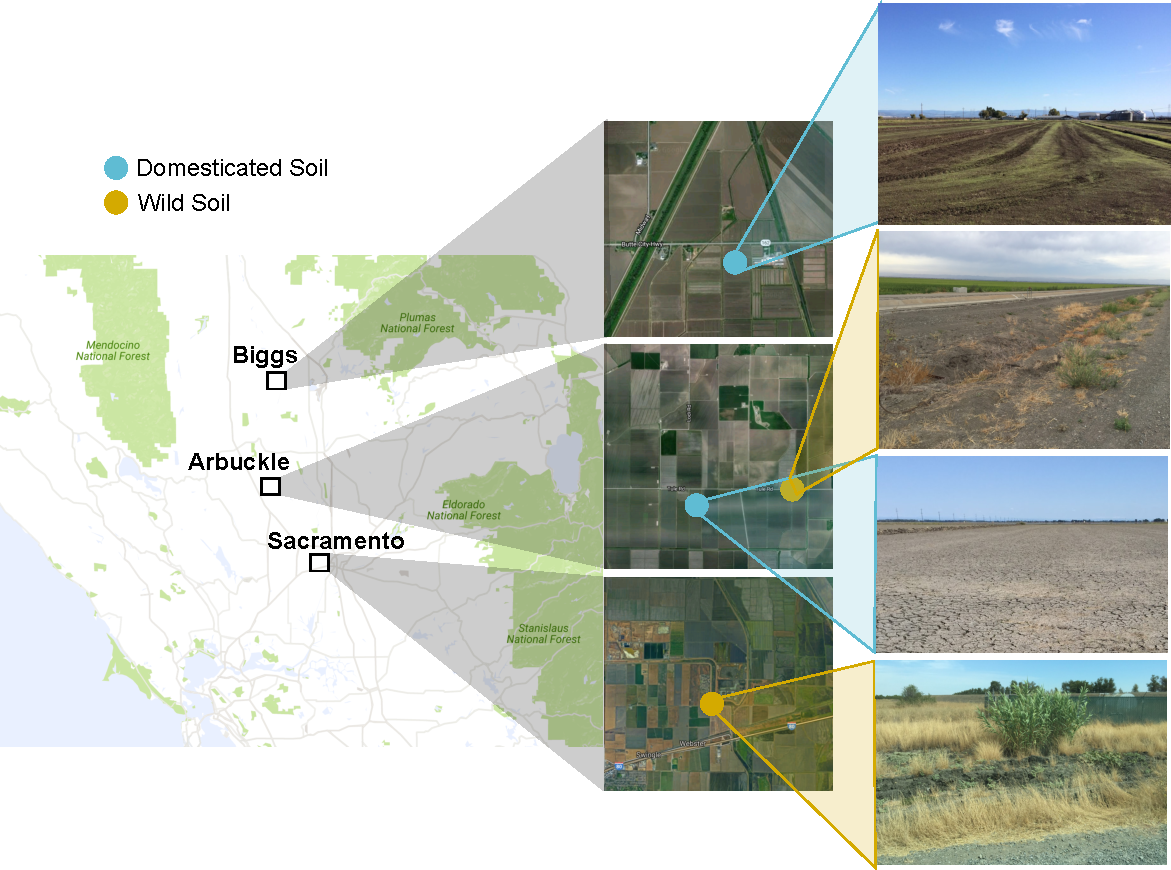
\includegraphics[width=6in]{Figures/figure2_s2}
\captionsetup{labelformat=empty}
\caption[Figure 3S2]{\textbf{Figure 3S2. Map of where wild and domesticated soils were collected.}}
\label{Figure 3S2}
\end{figure}

\newpage

\begin{figure}[h]
\centering
\includegraphics[width=4in]{Figures/figure2_s3}
\captionsetup{labelformat=empty}
\caption[Figure 3S3]{\textbf{Figure 3S3. Dispersion of beta diversities for each sample type from domesticated and wild soils.}}
\label{Figure 3S3}
\end{figure}
\chapter{Successional shifts in the root-associated microbiota throughout the life cycle of the crop plant \textit{Oryza sativa}}

Joseph Edwards\footnote[1]{Department of Plant Biology, University of California, Davis}, Christian Santos$^1$, Zach Liechty$^1$, Bao Nguyen$^1$, Nicole Chan$^1$, Eugene Lurie$^1$, and Venkatesan Sundaresan$^1$

\section{Abstract}
Much like how humans host a gut microbiota, plants assemble a root-associated microbiota which can aid the plant in assimilating nutrients, reducing susceptibility to pathogens, and alleviating the severity of abiotic stresses. Plants host microbiota in at least 3 distinct root-associated compartments: the rhizosphere, rhizoplane, and endosphere. It is unclear how the communities in these compartments shift over the course of the plant's life cycle or whether the transition to the reproductive phase has any effect on the root-associated microbiota. Here, we characterize the root-associated microbiota of the cereal crop \textit{Oryza sativa} over the course of 3 seasons. We found that the microbiota in each root-associated compartment shifts significantly over the life cycle of the plant and that these shifts are independent from the shifts in unplanted soil and are consistent from season to season. We found that the root microbiota shifts rapidly until the entry into the reproductive phase, whereupon the microbiota stabilizes. Using a machine learning framework, we identified taxa that were discriminant of plant age. We next investigated whether there exists a developmental stage-specific microbiota by sampling rice varieties with different developmental progression rates. Again using a machine learning approach, we were able to identify bacterial taxa whose abundance patterns are discriminant of plant developmental stage. These results indicate that changes in plant development either directly or indirectly impact the root-associated microbiota.

\section{Introduction}
Plants derive root-associated microbial communities from the soil which are inhabited by thousands of different species and strains of archaea and bacteria \cite{Lundberg2012,Bulgarelli2012,Peiffer2013,Edwards2015,Wagner2016}. Individual taxa within the root-associated microbiota have been found to be beneficial for plant growth and resistance to biotic and abiotic stresses \cite{Bulgarelli2013,Berendsen2012,Mendes2011}. In rice, we previously identified three spatially distinct root compartments with significantly different microbiota compositions: the soil adjacent to the root (the rhizosphere), the root surf,ace (the rhizoplane), and the root interior (the endosphere) \cite{Edwards2015}. It was found that each of these root-associated compartments have significantly different microbiota profiles from the communities in unplanted soil, thus indicating the roots enrich for subsets of the soil microbiota. This enrichment process and how the root-associated microbiota shift throughout the lifecycle of rice plants remain uncharacterized.

In humans, the successional shifts in the gut microbiota have been well studied from infancy into adulthood \cite{Koenig2011,Mueller2015,Backhed2015,Yatsunenko2012}. Newborns are characterized by a low diversity gut microbiota that increases with age \cite{Koenig2011}. The composition of the human gut microbiota shifts rapidly during the first three years of life, then stabilizes to become more like an adult microbiota after three years and these shifts correlate well with dietary intake \cite{Yatsunenko2012}. Whether a similar developmental  trend occurs within the root-associated microbiota of plants remains unclear. In this study, we detail the succession of microbial consortia in the three root-associated compartments of rice while being cultivated under field conditions. We also characterize how plant developmental progression is associated with the succession of various taxa.

\section{Results}
\subsection{Experimental Design and Sequencing}
We first were interested in monitoring how root-associated microbiotas shift throughout the life cycle of the rice plant under field conditions and whether changes in community profiles were consistent across multiple seasons. To do this, we collected the rhizosphere, rhizoplane, and endosphere microbiota samples from rice plants grown in a submerged commercial rice field in Arbuckle, California over the 2014 and 2015 seasons. In 2014, the field was sampled weekly until harvest, a total of 19 weeks with each time point consisting of 8 replicates. In 2015, because we were interested in the initial root colonization stage, we sampled every other day for the first 4 weeks of growth, thereafter sampling every other week until harvest. Each time point in 2015 consisted of 4 replicates. For each season, we collected bulk soil (i.e. soil from the submerged field where no roots were growing) until root growth made it impossible to locate soil unaffected by rice roots: around 4 weeks for the 2014 season and 6 weeks for the 2015 season.

PCR amplification and Illumina sequencing of the 16S rRNA gene was conducted to profile microbial communities present in each sample. Operational Taxonomic Unit (OTU) clustering was done at the 97\% threshold using the NINJA-OPS pipeline \cite{Al-Ghalith2016}. We detected a total of 24,048 OTUs across 1,290 samples with a total of 48,954,921 sequences. We removed a total of 276 detected OTUs matching mitochondrial or plastidial taxonomies. We then removed samples from our dataset with less than 1000 total reads. One difficulty of microbiome studies is to perform statistics on non-reproducible OTUs. We removed OTUs from our dataset that were not present in at least 5\% of the total samples. This step reduced our dataset to 8,554 OTUs for analysis.

\subsection{Microbiomes are shaped by distance from the root and plant age}
\begin{figure}[h]
\centering
\includegraphics[width=5in]{Figures/figure3_1}
\caption[Figure 4.1]{\textbf{The root-associated microbiota is differentiable by root compartment and plant age.} \textbf{(A)} Principal coordinate analysis (PCoA) of Bray-Curtis distances between samples colored by root-compartment. \textbf{(B)} The same plot as in A but colored by the age of the plant from which the samples were obtained. \textbf{(C)} The estimated slope of the second prinicipal coordinate of plot A as a function of plant age. We fit separate linear models to estimate that slope during the vegetative phase and the reproductive phase (defined as plants older than 63 days) for each compartment. The 2014 and 2015 seasons' data is included in plots A and B.}
\label{Figure 4.1}
\end{figure}

To understand the underlying driving forces of microbial community variation in our data, we used Principal Coordinates Analysis (PCoA) of Bray-Curtis distances. We found that samples from 2014 and 2015 display a spatial pattern of divergence along the first principal coordinate, where communities in bulk soil samples cluster on one end of the axis and endosphere communities cluster on the other (Fig. 4.1A). In agreement with our previous studies on the rice root-associated microbiomes \cite{Edwards2015}, perMANOVA of pairwise distances between samples indicated that microbial communities differed significantly between root-associated compartments (R2 = 0.23, P = 0.001). 

We next measured the effect of plant age on the root-associated microbiota. PerMANOVA of pairwise distances between samples revealed that plant age had a significant effect on the root-associated microbiota (R2 = 0.21, P = 0.001). We found that this effect was captured on the second principal coordinate of the PCoA plot (Fig. 4.1B). In the M206 cultivar, panicle initiation (entry into reproduction) occurs 56-63 days after germination \cite{Linquist2012}. We quantified the slope of the second principal coordinate in response to plant age for the vegetative stage (days < 63) and the reproductive stage (days >= 63) using a linear model. We found that in each root-associated compartment, the rate of change (i.e. the linear slope estimate) was reduced in the reproductive phase compared to the vegetative phase (Fig. 4.1C). This effect was consistent across the two seasons, suggesting that the root-associated microbiomes shift over the course of the plant's vegetative life cycle, but then stabilize at the onset of reproduction. Although we could not collect bulk samples during the reproductive phase of each season, we noticed a reduced rate of change among bulk soil samples compared to root-associated samples during the vegetative stage of growth. These results suggest that shifts in the root-associated microbiota over the course of the season is mainly driven by plant processes and not directly by changes in edaphic factors.

The multi-season sampling scheme of our experimental design allowed us to quantify the effect of seasonal variation on the root-associated microbiota. Although the root-associated microbiota varied significantly across the two seasons, the effect was small (R2 = 0.007, P = 0.001) compared to the other factors analyzed within this experiment. Together, these data suggest that the root-associated microbiota shifts in each root-associated compartment during the vegetative growth stage of the season and stabilizes upon entry into reproduction and that these patterns are consistent across multiple growing seasons.

\subsection{Microbiota shifts over the season are marked by increasing and decreasing relative abundance of specific phyla}
\begin{figure}[h]
\centering
\includegraphics[width=4.25in]{Figures/figure3_2}
% where an .eps filename suffix will be assumed under latex,
% and a .pdf suffix will be assumed for pdflatex
\caption[Figure 4.2]{\textbf{Shifts in the microbiota over time are associated with increasing and decreasing phyla.} \textbf{(A)} Bar plots of the top 11 phyla abundance over the course of the seasons in each compartment. Each bar represents 1 sample that was taken throughout the course of the growing season. The bars are ordered by the age of the plant as indicated by the colored points beneath each bar. Both the 2014 and 2015 data were used for this graph. \textbf{(B)} Beta regression coefficient estimates for microbial phyla that are either increasing (above 0) or decreasing (below 0) in relative abundance from the outside of the root to the inside of the root. \textbf{(C)} Beta regression coefficient estimates for microbial phyla that are increasing (above 0) or decreasing (below 0) in relative abundance over the course of the seasons in each compartment.}
\label{Figure 4.2}
\end{figure}

We next sought to characterize the specific phyla responsible for the significant differences between the root-associated compartments and how these various phyla changed in abundance over the lifecycle of the rice plants. Figure 4.2A shows the relative abundance for the top 11 most abundant phyla between the compartments and how their abundance changes over the course of the season. Because the Proteobacteria phylum contains a broad phylogenetic makeup and because Proteobacteria make up the vast proportion of the rice root-associated microbiota, we further dissected the Proteobacteria phylum into its respective classes for this analysis. To model increasing or decreasing relative abundance of individual phyla between the various root-associated compartments, we assigned each compartment a value relative to its spatial position: bulk soil was position 1, rhizosphere was position 2, rhizoplane was position 3, and endosphere was position 4. We modelled how phyla either increased or decreased between these positions using beta regression. Beta regression is used for modeling dependent variables which lie in the interval (0, 1) and is thus useful for modelling individual taxa as a relative proportion of the total microbial community. 

Using this method, we were capable of identifying phyla which significantly differ in spatial distribution from the exterior to the interior of the root. Figure 4.2B indicates the degree of change for phyla whose relative abundance were significantly different across the root-associated compartments. The phyla are ranked in terms of how pronounced the changes are between the exterior and interior of the root. Those taxa which have values below zero on the y-axis are higher in relative abundance outside of the root, while taxa with a value greater than zero are higher in relative abundance inside of the root. Our analysis revealed more taxa with negative trends from the outside to the inside of the root which is consistent with the hypothesis that the root is a selective niche unsuitable for the growth of a large array of soil microbes. Many of the phyla found to be significantly enriched from the soil to the root interior belong to various classes within the Proteobacteria phylum. We found both Spirochaetes and Fibrobacteres to increase in abundance from the outside to the inside of the root. Both phyla are known to degrade cellulose, thus it is probable that these microbes are using the root tissue as an energy source or as a molecular cue for colonization \cite{Kudo1987,Ransom-Jones2012}.

We performed the same type of analysis to identify phyla that significantly increased or decreased in relative abundance over the course of the growing season in each compartment. Figure 4.2C shows the result of this analysis where we display the top 15 phyla in each compartment which show the highest degree of change over the course of the season. Below zero on the x-axis represents phyla that were reduced in relative abundance over the season, while vlaues above zero represents taxa that increased in abundance over the season. The plant associated compartments showed similarities in phylum increase or decrease over the season. For instance, in the rhizosphere, rhizoplane, and endosphere Betaproteobacteria consistently decreased over the course of the season, while Deltaproteobacteria, Euryarchaeota, and Spirochaetes all increased. These results indicate that the relatively large variances partitioned to differences in microbial communities across the root-associated compartments and over the course of the growing season can be explained by significant proportional shifts in various phyla.

\subsection{The composition of the root-associated microbiota is an accurate predictor of plant age}

\begin{figure}[h]
\centering
\includegraphics[width=6in]{Figures/figure3_3}
\caption[Figure 4.3]{\textbf{Figure 3. Random forests model detect taxa that are accurately predictive of plant age.} \textbf{(A)} The result of predicting plant age using the sparse RF models for the 2014 and 2015 season. Each point represents a predicted age value, solid points were the samples on which the models were trained and the hollow points are samples in which the model never encountered during training. The solid black line represents the perfect fit line (i.e. if a sample were to be perfectly predicted, it would fall on this line). The dashed red line is a Loess regression curve fit to the predicted data from the 2014 season to show how the predicted values deviate from the real values. Each Loess curve is specific to the respective compartment from the 2014 data. These same curves are plotted along with the 2015 data to show that the areas of deviation from the perfect fit line are similar in the 2015 data. \textbf{(B)} The values of the bulk soil samples as predicted by the compartment specific RF models. The dashed red line is a linear fit for the bulk soil samples in each compartment's model showing how the predictions deviate from the perfect prediction line. \textbf{(C)} A heatmap representing the abundance profiles of the 66 most age discriminant OTUs in each compartment over the course of the season. \textbf{(D)} The number of models the OTUs belong to. A value of 3 means that the particular OTU was shared in all three compartment specific models. \textbf{(E)} Shows the slope estimates of the 10 shared OTUs between the compartments to indicate whether the OTU is increasing or decreasing as a function of plant age. The Order of the OTUs are shown in text next to the bars.}
\label{Figure 4.3}
\end{figure}

Because there were notable patterns of microbiota shifts throughout the growing season in each root-associated compartment, we next sought to identify patterns in the abundance of various taxa to discriminate the age of the rice plants. This posed a formidable difficulty due to the underlying structure of our data and the biology of the microorganisms we are studying. In our dataset exist the abundance of many thousands of detectable microbes. The abundance pattern over time is unique for each detected microbe and some of these abundance patterns are useful for predicting the age of the rice plant while others have little to no utility for this purpose. Because of this problem, we settled on using the Random Forests (RF) algorithm, a machine learning technique, to model the age of the rice plants by using the abundance patterns of various microbes \cite{Breiman2001}. The RF algorithm is particularly suited for this task because it can incorporate multiple variables for consideration (i.e. using multiple OTUs for predictions), it does not assume linear trends in the input data nor does it require the data to have a parametric distribution, and it can return the importance values for the input features (i.e. it outputs how useful an OTU was for creating an accurate model). 

To begin, we regressed the abundances of all 8554 detected OTUs in a training set of samples from each root-associated compartment separately as a function of plant age to form the ``full'' RF models. Because various taxa had different abundance profiles over time between each compartment (Figure 2A), we surmised that each compartment should be modeled separately in order to make the most accurate prediction. The training data for each compartment is a random selection of four of the eight replicates within each time point from the 2014 season. The full models are not optimally accurate because some OTUs which are not useful for predictions can introduce a significant amount of error. We then conducted 10-fold cross validation on each model while subsequently removing non-important OTUs in order to identify how many of the most important OTUs should be included in each model (Fig. 4S1). This analysis revealed a marginal decrease in cross-validation error when using greater than 66 of the most important OTU features for each model. Thus, for each root-associated compartment, we formed a ``sparse'' RF model using the most important 66 OTUs derived from each compartment's full RF model. The sparse models were used for downstream analysis and were not subjected to any further parameter optimization.

We used the sparse models to predict the ages of plants from our test set of samples consisting of the remaining samples from the 2014 season which were not included in the training of the model. Each model predicted the new data accurately (Fig. 4.3A), with the lowest adjusted R2 value being 0.89 in the test set of the 2014 endosphere data. The least accurate timeframe for each model was after 100 days where each model consistently under-predicted the plants' ages, perhaps due to the overall stability of the root associated microbiome during the reproductive phase. We also predicted the ages of plants from the 2015 season using these sparse model. Again, we found the models to be accurate in their predictions of plant ages based off of the 66 OTUs included in each model. We used the sparse models to predict the ages of bulk soil samples for the 2014 and 2014 seasons (Fig. 4.3B). Each model consistently mis-predicted the age of the bulk soil samples. These results suggest that the 66 age discriminatory OTUs included in each model fluctuate over the growing season, i.e. some OTUs have increasing abundance over the season while other have decreasing patterns (Fig. 4.3C), and these patterns of fluctuations are consistent across different seasons. Furthermore, the 66 OTUs in each model are specifically predictive for the root-associated compartments and not for bulk soil samples, suggesting that the fluctuations in abundance for the sets of 66 OTUs are driven by the host plants and are not directly influenced by edaphic factors.

We next examined the top age discriminatory OTUs in each sparse model. The models consisted of phylogenetically diverse sets of taxa (Fig. 4S2): included in the models were OTUs from 14 Phyla, 33 Classes, 55 Orders, and 58 Families. Interestingly there was minimal overlap in OTUs between the models: we found only 10 OTUs to be conserved between all three models, while 126 OTUs were unique to a model (Fig. 4.3D). Of the ten overlapping OTUs, only one had a significantly decreasing abundance over the season in each root-associated compartment while the remaining nine had significantly increasing abundance patterns over the season in each compartment (Fig. 4.3E). Only two of these OTUs were found to also have either a significant increasing or decreasing trend in the bulk soil samples. Taxonomically, 7 of the 10 OTUs belong to the Betaproteobacteria class, specifically within the orders of SBIa14 and Rhodocyclales. Taken together, these data indicate while a small set of OTUs are shared between the models, the models use a broad phylogenetic diversity of OTUs to discriminate plant age.

\begin{figure}[h]
\centering
\includegraphics[width=5in]{Figures/figure3_4}
% where an .eps filename suffix will be assumed under latex,
% and a .pdf suffix will be assumed for pdflatex
\caption[Figure 4.4]{\textbf{Hierarchical clustering of time points based upon abundance of the 66 most age discriminant OTUs in each compartment's sparse RF model.} Colors represent the developmental stage that the plants were in when sampled. The numbers represent that host plant's age at the time of sampling.}
\label{Figure 4.4}
\end{figure}

We were next interested in understanding how the various time points relate to each other in terms of microbial community structure. That is, do time points cluster based upon developmental stages? To address this question, we performed hierarchical clustering using the 66 most age-discriminant taxa in each compartment (Fig. 4.4). The particular variety that was included in this study, M206, starts transitioning to the reproductive phase around 56 to 63 weeks after germination. In each compartment we found clear clustering of the time points during the vegetative phase. Consistently across each compartment, we found that the samples taken on day 56 through 70 cluster together. This is a transition time for the rice plants where they are switching from vegetative to reproductive growth. Interestingly, this transitory cluster falls closer to the reproductive or vegetative time points depending on the observed compartment. For instance, in the rhizosphere the transitory time points cluster with the vegetative samples and in the endosphere and rhizoplane the transitory time points cluster with the reproductive time points. This may suggest that the endosphere and rhizoplane microbiomes are the first to be affected by the transition to reproduction while the rhizosphere follows suit later.	

\subsection{Developmental stage is a driver of microbiota succession}
\begin{figure}[tbh]
\centering
\includegraphics[width=6in]{Figures/figure3_5}
% where an .eps filename suffix will be assumed under latex,
% and a .pdf suffix will be assumed for pdflatex
\caption[Figure 4.5]{\textbf{Varieties with different developmental rates have different microbiota progressions.} \textbf{(A)} The developmental stage of the tested varieties as a function of plant age. We devised a numerical system for developmental progress based up morphological features indicative of developmental stage. \textbf{(B)} PCoA of the 2016 data indicating root-associated compartment and plant age are major determinants of microbiota structure. \textbf{(C)} Linear slope estimates for the principal coordinate 2 in panel B as a function of plant age for each variety and each compartment. A higher slope indicates that the microbiota is progressing faster along PCo2 as a function of plant age. \textbf{(D)} The predicted age of the 2016 data as predicted by the age discriminant sparse RF models. The solid black line is the perfect fit and the red dashed lines are the Loess curves calculated in Fig. 4.3A. \textbf{(E)} The inverse of the mean squared residual errors from panel D. A larger value means the model had more accurate predictions for the respective set of samples.}
\label{Figure 4.5}
\end{figure}

Our sparse models appear to be detecting shifts in the root-associated microbiota that correlate with developmental shifts in the rice plants. However, shifts in plant development also co-vary with shifting climatic and edaphic factors which may have indirect effects on the microbiota through various plant responses, thus making these factors difficult to uncouple from the effect of plant developmental stage on the shifting root-associated microbiota. Because our study was confined to one commercial field, we were limited to studying the dynamics of one rice variety throughout the 2014 and 2015 seasons which was synced in its developmental progression. To have a better idea of whether plant developmental stage significantly impacts the root-associated microbiota, we needed to un-sync plant age from developmental progression. In order to achieve this goal, we decided to grow rice varieties with different developmental rates in the same field in Arbuckle, CA. Plant genotype, while significant, has a relatively small effect on the root-associated microbiota compared to other environmental effects (such as drought), thus we chose 4 varieties from the tropical \textit{Japonica} sub-species of \textit{Oryza sativa} for this study, all with different developmental progression rates (Figure 5A). Kitaake, a variety often used by research labs because of its relatively fast generation to generation time, reaches the flowering stage faster than the rest of the included varieties. We included the California varieties M206 and M401 into this study. M206 is the variety that we have previously been studying in the Arbuckle field and the variety for which the sparse RF models were generated. Although M401 and M206 reach the panicle initiation stage around the same time, M401 has a much later heading data. We also included the variety Nipponbare, which reaches panicle initiation later than the rest of the varieties, but flowers within the same timeframe as M401. These varieties were water seeded in the Arbuckle field in a complete randomized block design (Figure 5A). We sampled plants within each plot every two weeks throughout the season, collecting rhizosphere, rhizoplane, and endosphere fractions from the plant roots. Our field design allowed us to also collect bulk soil samples throughout the entirety of the season as compared to the 2014 and 2015 seasons, which restricted our soil sampling due to the invasiveness of the rice roots. 

The data from the 2016 season had similar trends as exhibited in the 2014 and 2015 seasons. The root-associated compartments hosted distinct microbiotas (Fig. 4.5B, R2 = 0.27, P < 0.001) and the microbiota varied significantly due to plant age (Fig. 4.5B, R2 = 0.17, P < 0.001). We found that genotype had a very small overall effect on the root-associated microbiota (R2 = 0.01, P < 0.001). This level of variance is smaller than what we have previously detected in rice \cite{Edwards2015}. In our previous study, we grew 6 different cultivars in the greenhouse: 2 temperate \textit{Japonica}, 2 \textit{Indica}, and 2 \textit{Oryza glaberrima}. Our current study only used varieties within the temperate \textit{Japonica} clade, thus we expect that the reduced genetic diversity within this experimental population led to lower levels of microbiota variation compared out the previous study. We noticed that there was a significant statistical interaction between plant age and genotype (R2 = 0.05, P < 0.001), suggesting that the trends in microbiota shifts over the season differ depending on the rice genotype. To further inspect this observation, we calculated the slope of the second principal coordinate of Fig 5B as a function of plant age. We used the second principal coordinate because it was the axis best differentiating between plant age. We hypothesized that if plant developmental rate were to have an effect on the root associated microbiota, then the faster developing varieties would have steeper slopes than the slower developing varieties. Indeed, we found that Kitaake had the steepest slope in each compartment, while M206 and M401 have similar slopes and Nipponbare had the most gradual slope in each compartment. Bulk soil, however, had a much reduced slope over the season and is almost flat. Taken together these results indicate that microbiota shifts throughout the season are directly driven by the host plant and the rate of these shifts correlate with the developmental progression rate of the host plant.

\subsection{Developmental stage is a driver of microbiota succession}
\begin{figure}[tbh]
\centering
\includegraphics[width=3in]{Figures/figure3_6}
% where an .eps filename suffix will be assumed under latex,
% and a .pdf suffix will be assumed for pdflatex
\caption[Figure 4.6]{\textbf{Random forests model detect taxa that are accurately predictive of plant developmental stage.} \textbf{(A)} Results of the model after predicting developmental stages of the samples taken from the 2016 season in each compartment plotted as a function of plant age. The different varieties separate similar to the pattern exhibited in Figure 5A. \textbf{(B)} The abundance profiles of the top 10 most developmental stage discriminant taxa in each compartment over the course of the 2016 season.}
\label{Figure 4.6}
\end{figure}

We next used the sparse RF models to predict the age of samples taken from the 2016 season (Fig. 4.5D). The models were remarkably accurate at predicting the ages of plants from the 2016 season despite the differences in the developmental progression rates of the genotypes. We calculated the mean squared error (MSE) of residuals for each genotypes predicted values by the compartment specific sparse RF models (Fig. 4.5E). In the case of the rhizosphere and rhizoplane, the age of the M206 genotype was most accurately predicted by the models (it was the second most accurately predicted variety using the endosphere models). The original models were trained on data collected from M206 during the 2014 season. These results suggest that the accuracies of the models are affected by the differences between the genotypes likely due to variation in developmental progression rate. 

To have a better understanding of which microbes are associated with the various developmental stages, we formed new RF models for predicting plant developmental stage rather than plant age. Development in plants is a continuous process marked by numerous stage-specific morphological features. We monitored the developmental stage of the genotypes throughout the season assigning a numerical value from 1-27, with a value of 1 corresponding to a recently germinated seeding and 27 corresponding to a senescent plant. Panicle initiation corresponded to a value of 18, thus a plant that is transitioning to the reproductive phase has a value of 18 or higher and a plant in the vegetative phase has a value of 17 or lower. We followed the same approach as previously mentioned to develop the RF models. Briefly, we trained full RF models in each compartment where we regressed the full dataset of OTUs against the developmental stage number for a training set of samples. From these full models, we sequentially removed OTUs of lower importance while performing 10-fold cross validation. We found that the models were near peak accuracy when including 29 of the most important OTUs for each compartment (Fig. 4S3). With these 29 most-important OTUs, we developed sparse RF models that modelled the microbiota as a function of plant developmental stage. When the predicted values of plant developmental stage were plotted as a function of the plant's chronological age, we found that the predictions accurately matched the developmental progressions that we witnessed in the field (compare the prediction plot in Fig. 4.6A to the plot of witnessed developmental progressions in Fig. 4.5A). These results indicate that the sparse RF models were able to detect shifts in the microbiota that correlate with developmental shifts in the plant. The abundance profiles for each the top 10 most important OTUs for each compartment's model's accuracy are plotted in Fig. 4.6B. The developmental stage sparse RF models used less OTUs than the plant age models to make accurate predictions. This suggests that the total root-associated microbiome is more affected by the chronological age of the plant rather than the plant's developmental stage.

\section{Discussion}
Annual plants quickly undergo large shifts in morphology and physiology throughout their lifecycle \cite{Freeling1990,Moldenhauer}. Developmental shifts are accompanied by different nutritional requirements and source sink relationships \cite{Ishimaru2013,Tegeder2010} which in turn could affect the compositional profile of the root-associated microbiota. Here we have detailed how the root-associated microbiota shift throughout the life cycle of rice plants growing in a single field in Arbuckle, CA. We found that the microbiota shifts significantly over time, with most of these shifts happening in the vegetative phase of developmental and a stabilization of the microbiota occurs after the entry into the reproductive phase. We found that there are large shifts in various phyla throughout the season. Members of the Deltaproteobacteria class predominantly increased over the season and members of the class Betaproteobacteria predominantly decreased over the season. We found that these patterns held over multiple seasons and that seasonal effects were of minimal importance on the overall root-associated microbiota. The bulk soil community members are relatively stable compared to the root-associated microbiota, suggesting that the plant non-randomly controls the fluctuating abundances of various taxa throughout the season. We found that the microbiota is predictive of plant age by fitting sparse random forests models to each compartment. These models identified many plant age discriminant microbial taxa which reproducibly changed in abundance over the course of the season. The mechanisms by which plants control the structure of their root-associated microbiota is unknown. Using cultured representatives from these age-discriminant microbial taxa in controlled inoculation experiments could help elucidate these processes and may suggest various roles for members of the root-associated microbiota on host health. 

From our initial results, it remained unclear whether plant developmental stage was indeed a regulator of the root-associated microbiota structure. A recent study claimed that the entry into flowering likely has no effect on the root-associated microbiota \cite{Dombrowski2016}. The authors conducted a clever experiment by growing a very early flowering \textit{Arabis alpina} mutant, \textit{perpetual flowering1} (\textit{pep1})\cite{Wang2009}, along with wild type Arabis alpina. They collected samples from the rhizosphere and endosphere of each genotype after 6, 12, and 28 weeks of growth (the pep1 mutant flowers after 12 weeks). They found no significant differences in the microbiotas taken from the flowering mutant and the still vegetatively growing wild type plants. They did, however, find significant differences in root-associated microbiotas between the different time points. These results led the authors to conclude that the root-associated microbiota is affected by plant residence time (i.e. the chronological age of the host plant) but not the developmental stage. \textit{Arabis alpina} (a wild \textit{Arabidopsis thaliana} relative) is a perennial plant, and is thus physiologically distinct from rice plants. We tested the hypothesis ourselves of whether fluctuations in the microbiota are correlated with different developmental stages by growing several rice varieties with different flowering times under field conditions and sampling their root microbiota throughout the growing season. We found that the progression of the microbiota throughout the season is correlated with the developmental progression of the plant and that these progressions are not found in the microbiota of unplanted soil. We developed models to predict the developmental stages of the plants using the abundance of various members within the plants' root-associated microbiota. From these models we were able to extract various microbes whose abundance profiles are predictive of plant developmental stage. Isolating these candidate microbes in pure culture would allow for a deeper investigation of how host plants communicate with their microbiota during various developmental and physiological states.

The random forests models trained to discriminate plant age detected more microbes than the random forests models trained to predict plant development. This discrepancy is indicative that plant age has a larger impact on the overall structure of the root-associated microbiota than plant developmental stage, yet plant developmental stage is still an important factor for differentiating the root-associated microbiota. Our results are clearly different than the aforementioned study that found no microbes to be affected by plant developmental stage. There are several likely causes for this discrepancy. Arabis alpina is a wild perennial plant species and rice is a domesticated annual crop species. One hallmark trait of cereal domestication is the selection for varieties with larger sink sizes in the seed \cite{Ishimaru2013}. For instance, in wild grass species, source carbohydrates are more evenly distributed to various sink tissues in the plant than domesticated cereals, where the seeds are a predominant sink \cite{Shomura2008,Ishimaru2013}. The discrepancy between sink-source dynamics in these two host plants could, at least partially, explain why our study detected shifts in the microbiota due to developmental stage while it was undetected in Arabis. In rice, accumulation and storage of carbohydrates in the stems occur until the onset of reproduction, after which internal signals program the host plant to begin repartitioning carbohydrates to the developing panicle and to the filling grain \cite{Slewinski2012,Scofield2009}. These host signals, along with the shifting nutritional needs at this stage could explain the stabilization in the microbiota that occurs at the onset of reproduction. Here we have a provided one of the first links between host plant development and composition of the root-associated microbiota. Understanding the physiological, molecular, and developmental signals from the host plant that affect the root-associated microbiota may unlock the use of microbes to boost plant performance and yield.
	
\section{Materials and Methods}
%
\subsection{Plant growth and sampling during the 2014 and 2015 seasons}
%
We collected samples from a commercially cultivated rice field in Arbuckle, CA. In both seasons the field was water seeded in early May. Water seeding is conducted by first preparing the field by removing winter vegetation, disking the soil to produce baseball sized clods, applying nutrients, and then flooding \cite{Hardke}. The rice seeds are soaked in water overnight and then loaded into an aircraft where they are then applied aerially to the field in an even density. For this particular field, the farmer grew the M206 cultivar, a medium grained California variety that has an average heading date of 86 days after germination \cite{Linquist2012}. We began sampling plants 7 days after the fields were seeded, which coincided with the emergence of the seminal roots. In the 2015 and 2016 seasons we restricted our area of sampling to a 150 x 150 foot plot. Within this plot we would sample plants from random locations. Our sampling occurred as previously described. Using gloved hands, would scoop under the root mass to separate the plant from the ground. Grabbing the plant by the base of the stem, we would then shake the plant to remove loosely attached soil from the roots. We would then place the roots with tightly adhering soil into 50 mL Falcon tubes with 15 mL autoclaved phosphate buffered saline (PBS) solution. We would then bring the samples back to the laboratory at UC Davis. We collected bulk soil samples as the season allowed. During the later parts of the season it became impossible to find soil samples unaffected by rice roots.

\subsection{Plant growth during the 2016 Season}%
We grew various cultivars in the same field in Arbuckle, CA for the 2016 season. Briefly we designed a fully randomized block design to grow these varieties in 1 x 1 m plots in quadruplicate. We left 0.5 m wide walking lanes between each plot which subsequently allowed us to sample bulk soil throughout the course of the growing season. To be consistent with the previous years' methods, we water seeded these varieties. This entailed soaking the seeds in a 2\% bleach solution for 4 hours to remove the risk of the field being contaminated \textit{Fusarium moniliforme}, a seed borne fungal pathogen that causes the disease Bakanae. The seeds were then washed 3 times with sterile water and soaked overnight. We then hand seeded each plot at similar density as what the farmer had applied in previous seasons. At each timepoint the plants were sampled as previously described and transported to the lab for further processing. The plants used for sampling during this season were dissected to score various developmental stages between the cultivars \cite{Moldenhauer}.

\subsection{Separation of the root-associated compartments and DNA extraction}
%
The root associated compartments were separated as previously described \cite{Edwards2015}. The roots with soil attached were vortexed in PBS solution and 500 uL of the resulting slurry was used for DNA extraction. The roots were cyclically washed in fresh PBS solution until no soil particles were visible in the solution. The roots were then placed into fresh PBS and sonicated for 30 s to remove surface cell layer of the roots. The resulting slurry was centrifuged down to concentrate the biomass and then used as the rhizoplane fraction for DNA extraction. The remaining roots were sonicated twice more, refreshing the PBS solution at each stage, and then ground in the bead beater. The resulting solution was used for DNA extraction as the endosphere fraction. All DNA extraction was performed using the MoBio Powersoil DNA isolation kits.

\subsection{PCR amplification and sequencing}
%
We amplified the V4 region of the 16S ribosomal RNA gene using the universal 515F and 806R PCR primers. Both our forward and reverse primers contained 12 base pair barcodes, thus allowing us to multiplex our sequencing libraries at well over 150 libraries per sequencing run. Each library was accompanied by a negative PCR control to ensure that the reagents were free of contaminant DNA. We purified the PCR products using AMPure beads to remove unused PCR reagents and resulting primer dimers. After purification, we quantified the concentration of our libraries using a Qubit machine. Our libraries were then pooled into equal concentrations into a single library and concentrated using AMPure beads. The pooled library then went through a final gel purification to remove any remaining unwanted PCR products. Pooled libraries were sequenced using the Illumina MiSeq machine with 250 x 250 paired end chemistry. 

\subsection{Sequence Processing, OTU clustering, and OTU filtering}
%
The resulting sequences were demultiplexed using the barcode sequences by custom Python scripts. The sequences were quality filtered and then assembled into full contigs using the PandaSeq software \cite{Masella2012}. Any sequences containing ambiguous bases or having a length of over 275 were discarded from the analysis. The high-quality sequences were clustered into operational taxonomic units (OTUs) using the Ninja-OPS pipeline \cite{Al-Ghalith2016} against the Green Genes database \cite{DeSantis2006} and then assembled into an OTU table. This OTU table was filtered to remove plastidial and mitochondrial OTUs and filtered to remove OTUs that occur in less than 5\% of the samples. This process removed the total OTU count from 24,048 to 8,554 taxa. The resulting 8,554 taxa were used for the analysis.

\subsection{Statistical Analysis}
%
All statistical analyses were conducted using R version 3.1 \cite{RCoreTeam2016}. Unless otherwise noted, we determined statistical significance at $\alpha$ = 0.05 and, where appropriate, corrected for multiple hypothesis testing using the false discovery rate method. Shannon diversity was calculated using the diversity() function, PCoA analyses were conducted using the capscale() function, perMANOVA was conducted using the adonis() function, and community structure variability was measured using the betadisper() function all from the Vegan package \cite{Oksanen2013}. Linear models were run using the lm() function and ANOVA was run using the aov() function. Beta regression was used to model proportion of any given phylum ($\mu_p$) as function of distance from the root ($x_2$) using the betareg() function from the BetaReg package \cite{Cribari-Neto}. To do this, we assigned each compartment a value from the outside to the inside of the root: bulk soil had a value of 1 and endopshere had a value of 4. The model is described by the equation
\begin{equation}
    g(\mu_p) = \beta_1 + \beta_2 x_{p2}
 \end{equation}
 We also used beta regression to model trends in proportions for a given phylum ($p$) in a given compartment ($c$) as a function of host plant age ($x_2$) using the equation
 \begin{equation}
 	g(\mu_{pc}) = \beta_1 + \beta_2 x_{pc2}
 \end{equation}
 For each model, we used a logit link function. Random forests models were generated and analyzed using the randomForest package \cite{Liaw2015}. All graphs and plots were generated using the ggplot2 package \cite{Wickham2009}. R notebooks for the full analyses can be found on GitHub (https://github.com/bulksoil).

\newpage

\begin{figure}[h]
\centering
\includegraphics[width=5in]{Figures/figure3_s1}
\captionsetup{labelformat=empty}
\caption[Figure 4S1]{\textbf{Figure 4S1. Cross validation error of models predicting plant age while sequentially removing less important OTUs for model accuracy.} This analysis revealed that 66 of the most important OTUs should be included for the models to be the most accurate for predicting plant age.}
\label{Figure 4S1}
\end{figure}

\newpage

\begin{figure}[h]
\centering
\includegraphics[width=6in]{Figures/figure3_s2}
\captionsetup{labelformat=empty}
\caption[Figure 4S2]{\textbf{Figure 4S2. The orders of the 66 most important OTUs used in the sparse RF models predicting plant age.}}
\label{Figure 4S2}
\end{figure}

\newpage

\begin{figure}[h]
\centering
\includegraphics[width=4in]{Figures/figure3_s3}
\captionsetup{labelformat=empty}
\caption[Figure 4S3]{\textbf{Figure 4S3. Cross validation error of RF models predicting plant developmental stage while sequentially removing less important OTUs for model accuracy.} This analysis revealed that 29 of the most important OTUs should be included for the models to be the most accurate for predicting plant age.}
\label{Figure 4S3}
\end{figure}
\chapter{Conclusion}
It has been postulated that microbiota associated with multicellular organisms act as second genomes for their hosts \cite{grice2012human}. That is, the collective genomes of the microorganisms within a microbiome provide functions that are not encoded within the host organism’s genome. Indeed, many parallels can be drawn between the genome of the host and the composition of the microbiota. The host’s genome and microbiota are both structured into individual, non-overlapping units where the genome contains genes and the microbiota contains individual microbial taxa. Each unit within the genome and microbiota can be “expressed” at different levels depending on various environmental stimuli where genes are transcribed into mRNA of different abundances and individual microbial taxa multiply to have different cell counts. Moreover, trans-regulation occurs in both gene expression and microbial cell pro{}liferation. For instance, gene x may regulate the expression of gene y through binding to its promoter and microbe a may regulate the proliferation of microbe b by providing it critical nutrients. A striking difference between the innate genome and the second genome, however, is the nature by which they are acquired. Genomes are hereditary, being passed along from parent to offspring. A microbiota, however, is acquired from the environment. In the case of a plant, the root microbiota is primarily derived from the soil \cite{Zarraonaindia2015}. Characterizing the contents of the plant’s second genome and understanding the rules governing its acquisition are the primary foci of this dissertation.

\section{Chapter 1}
In the first chapter, I described the general characteristics of rice root-associated microbiota. We began by quantifying how microbial community profiles differ as a function of distance to the root. We detailed the microbiota within three root-associated compartments: the rhizosphere (soil tightly adhering to the root), the rhizoplane (the root surface), and the endosphere (the interior of the root). We found all three of these compartments to host distinct microbial communities and that each community is also distinct from the microbiota of unplanted soil. The rhizoplane and endosphere communities had lower microbial diversity compared to the rhizosphere and bulk soil, suggesting that there is a niche specialization for the microbiota in these root-associated compartments. We next characterized the effect of soil type on the root-associated microbial communities of rice. We found that soil originating from various rice fields host distinct sets of microbes and this in turn determines the subset of microbes that can colonize the roots of plants growing within these soils. We found similar trends in the trends in the abundance of various phyla across the root-associated compartments of plants grown in the different soils. For instance, in each soil Acidobacteria microbes have a decreasing abundance from the soil to the inside of the root, while Proteobacteria have an increased abundance inside the root and lower abundance in the soil. We also found that soil communities can be affected by agricultural practice. Specifically, root-associated microbiota are differentiable based upon whether the plants were grown under organic or conventional cultivation. We next characterized how the microbiota differs between various domesticated rice varieties. We profiled the microbiota from several cultivated varieties of two domesticated rice species, \textit{Oryza sativa} and \textit{Oryza glaberrima}, and found that rice genotype has a very minimal (although significant) effect on the root-associated microbiota. Many of these results have been corroborated by similar studies in other plant models. The results of the experiments are summarized in the visual model below. The model can be interpreted as such:
\begin{itemize}
\item Different soils host different consortia of microbes which can depend on geography or agricultural practice. This is indicated by different colors between the soil microbiota in the model.
\item Rice plants assemble a root-associated microbiota from the soil in which the plants are growing and this microbiota resembles the parent soil. The microbes that assemble on the inside of the root are much reduced subset of the soil community. This is indicated by the lighter color within the circle of the root-associated microbiota in the model.
\item Rice genotype has only a small effect on the root-associated microbiota even though much visible phenotypic diversity exists between the varieties. In the model, this is portrayed as the different hues in color between the different varieties. Please note that they are still reminiscent of the original hue of the parent soil in which the plants are growing.
\end{itemize}

\begin{figure}[h]
\centering
\includegraphics[width=5in]{Figures/figurec_1}
\caption[Figure 5.1]{\textbf{Model depicting host and environmental factos affecting the root-associated microbiota}}
\label{Figure 5.1}
\end{figure}

\section{Chapter 2}
In the second chapter, I characterized how the rice root-associated microbiota differs from other plants' microbiotas. We were perplexed that genotypic variation within two species of the Oryza genus only had a small impact on the root-associated microbiota. The varieties that we used for our experiment had distinct morphological traits that made each variety easily identifiable, yet their root microbiota was overall remarkably similar. We hypothesized perhaps there was a large conservation of root-associated microbiota across different lineages of flowering plants. We tested this hypothesis by first compiling published data from other plant root-associated microbiota studies that used similar methods to the methods in my first chapter. We found that each plant species assembles a distinct microbiota, but that his effect is confounded by the studies occurring in different geographic regions and environments. The rice microbiota was an outlier in this analysis, potentially due to its semi-submerged growth habit. We therefore collected and analyzed the root-associated microbiotas of three separate host plants growing in the same semi-submerged conditions as rice. We found that the microbiota from these plants, all of which are common rice paddy weeds with broad distributions across the United States, have distinct sets of microbial taxa colonizing their root-associated compartments. Rice, however, hosted an outlier microbiota compared to the other plants. The microbiota of rice plants were enriched for methane-producing microbes while the other plant species hosted microbiotas enriched for methane-utilizing microbes. It was also found from this experiment that the rice rhizosphere microbiota composition is notably similar to the microbiota from unplanted agricultural soil. We attributed this effect to continuous and intensive cultivation of rice which may in turn ``domesticate'' the soil microbiota to be more like the rhizosphere microbiota from rice. I have summarized the results of this analysis in the visual model below:

\begin{itemize}
\item The composition of the soil microbiota in which the different host plants are growing is represented by the orange box.
\item Each species assembled a significantly different microbiota as represented by the different colors of the root-associated microbiota circles for each host species. Notice that the different rice genotypes host a microbiota that is more similar to the hue of the bulk soil than the microbiotas of the other included host plant species.
\item The differences in microbiota composition between the different host species may have functional and environmental impacts, illustrated by the finding that the rice plants host more methanogenic microbes than the other host species in the same field.
\end{itemize}

\begin{figure}[h]
\centering
\includegraphics[width=6in]{Figures/figurec_2}
\caption[Figure 5.2]{\textbf{Model depicting the impact of host plant genotypic diversity on the root-associated microbiota}}
\label{Figure 5.2}
\end{figure}

\section{Chapter 3}
In the third chapter, I characterized how the root-associated microbiota changes throughout the lifecycle of the rice plant. Plants undergo large morphological and physiological shifts throughout their life cycle which in turn have stage-specific nutritional and environmental demands \cite{Ishimaru2013}. We sampled the microbiota of rice plants growing in single field in California over the course of three seasons. Remarkably, we found there to be only a small amount of variation across the seasons. In each compartment, we found that the microbiota progressively shifts throughout the growing season, especially during the vegetative phase of growth. These shifts are most pronounced in decreasing abundance of Betaproteobacteria and increasing abundance of Deltaproteobacteria over the course of the season. Upon the entry into the reproductive stage of development, we found that the overall composition of root-associated microbiota stabilizes. This shift appeared to be faster in the endosphere and rhizoplane than in the rhizosphere. In the first two seasons of our experiment, we were unable to definitively attribute the shifting microbiota to plant developmental progression in the first two seasons of our trial because all of the sampled plants were synchronized for developmental progression. There are environmental and edaphic factors that fluctuate over the season and there is also a possibility that the microbes require a certain amount of time to stabilize independent of plant developmental stage. To examine the effect of plant developmental stage on the root-associated microbiota independent of plant age and fluctuating environmental and edaphic factors, we grew different varieties that progress through development at different rates. Indeed, we found that faster progressing genotypes had faster shifting microbiotas. By using a machine learning approach, we were able to identify individual microbes whose abundance are descriptive of developmental stage. I have summarized our model for root-associated microbiota shifts over the lifecycle of the rice plant in a visual model below.

\begin{itemize}
\item The microbiota shifts in a gradient over the course of the season as mimicked by the hue of the horizontal bar shifting from the beginning of the season to the end.
\item The microbiota shifts during the vegetative phase of the rice plant's life (i.e. the seedling and tillering stages) until the onset of reproduction where the microbiome remains relatively steady. This pattern is denoted by the shifting hue of the horizontal bar during the vegetative phase which becomes steady at the onset of the panicle initiation stage.
\end{itemize}

\begin{figure}[h]
\centering
\includegraphics[width=5in]{Figures/figurec_3}
\caption[Figure 5.3]{\textbf{Model depicting the dynamic shifts in the microbiota over the course of a growing season as a function of plant developmental stage}}
\label{Figure 5.3}
\end{figure}

\section{Future Directions}
Here, I have described the composition, spatial structure, and acquisition of the rice root-associated microbiome, or the ``second genome'' of the plant. As I described earlier in this section, conceptual similarities exist between host-associated microbiota and genomes; however, it is unlikely that the similarities are limited to the examples above. Therefore, in moving forward with understanding the root-associated microbiota, it will be important for researchers to combine both ecological and genetic frameworks.

The functional impact of the microbiome as a whole on the host plant remains unknown. This is in large part because researchers have a lacked a controlled system to measure the traits of plants with and without a microbiota. This difficulty was overcome in animal systems by rearing germ-free mice (i.e. mice un-colonized by microbiota) which researchers could inoculate controlled microbial communities into and measure resulting traits \cite{Turnbaugh}. There is an ongoing effort by plant researchers with initial success to develop a similar axenic system to test how microbial consortia may impact plant traits (C. Santos, UC Davis, personal communication). 

To better understand how individual members of the root-associated microbiota impact plant fitness, an approach akin to ``mutagenesis'' could be used. Researchers are employing a relatively new approach to studying host-associated microbiota by introducing synthetic communities of cultured isolates to plant tissues \cite{bodenhausen2014synthetic,bai2015functional,lebeis2015salicylic}. It is conceivable that researchers could study the impact of a single microbial taxon on a given host trait by excluding it from an introduced synthetic community in a germ-free system, thus ``knocking out'' the microbe from the system. To extend this concept, a researcher could idenitify epistatic relationships between individual microbial taxa within a controlled system.

An alternative approach to discovering how individual microbial taxa affect plant host traits is by using an approach similar to a genome wide association study (GWAS). In GWAS, a genetic population with genotypic and phenotypic variation is used to correlate genetic variants (typically single nucleotide polymorphisms) with variation within phenotypic traits \cite{hardy2009genomewide}. Using this approach, it is possible to discover genes which may be responsible for a certain trait. One can imagine an example where a researcher can grow isogenic plants in different soils with sufficiently disparate microbiota to correlate the abundance of various microbes with plant traits. For example, if a researcher were to grow a single rice cultivar in 100 different salinity-stricken soils and measure the productivity of the plants, the researcher could correlate single microbial taxa or groups of taxa that may help plants survive under salt stress.

What result does microbiome hybridization have on the plant? In genetics, heterosis is a phenomenon where the resulting offspring of a genetic cross displays traits with better quality than either of the parents used to make the cross \cite{stuber1992identification}. If two soils with significantly different microbiota were to be mixed, would plants growing in the mixed soil display improved traits? If this were the case, could dominant and recessive microbes be identified that are responsible for the trait?

I hope I have made a persuasive case that using concepts derived from genetics as an approach for understanding root-associated microbiota provides a logical path forward with many interesting opportunities. The outcome will benefit not only researchers by accelerating progress in this field, but will be instrumental in unlocking the latent benefits of root-associated microbiota for crop growth and yield.


\bibliography{dissertation}

% The UMI abstract uses square brackets!
\UMIabstract[Soil microbes are important mediators of plant nutrition, growth, and resistance to biotic and abiotic stresses, thus understanding the composition and dynamics of plant root-associated microbial communities is of importance to scientists and farmers. Plants acquire root-associated microbiota that are distinct from that of the surrounding soil. In this thesis I detail general characteristics of the rice root-associated microbiota. 

In the first chapter I introduce the importance of both animal and plant microbiota and I discuss the technological breakthroughs that have allowed scientists to study complex microbial ecosystems. 

In the second chapter, I present the results of a study characterizing the rice root-associated microbiota across three root compartments: the soil adjacent to the root (the rhizosphere), the root surface (the rhizoplane), and the root interior (the endosphere). I present how the composition of the microbiota in these compartments varies across soil type, cultivation practice, and host plant genotype. 

In the third chapter, I present the results of a study characterizing the rice root-associated microbiota compared to diverse species of both crop plants and native plants growing in the same environment as rice. The results suggest that rice assimilates a unique root-associated microbiota and that plant phylogenetic variation cannot fully explain microbiota variation between the tested host plants. A comparison of the root-associated microbiomes of rice with microbiota of soil from cultivated fields and non-cultivated soils, suggests that rice cultivation changes the overall soil microbiome in rice fields not only through agricultural inputs and water submergence, but also through specific enrichment of microbial taxa by rice plants. 

In the fourth chapter, I demonstrate how the rice root-associated microbiota shifts across the lifecycle of the host plants under field conditions. We find that the composition of the microbiome shifts throughout vegetative growth until the initiation of reproductive growth, whereupon the microbiome stabilizes. These results suggest that plants select for different microbiota as they undergo developmental changes from germination to reproduction. 

I present concluding remarks on the various models of microbiota acquisition and discuss future implications of this research in the fifth and final chapter of this dissertation.] 

\end{document} 